\section{I buoni ordinamenti}
Il nostro prossimo obiettivo è definire e studiare la classe dei \vocab{numeri ordinali}. Questa può essere pensata come la più vasta classe
- dotata di un ordinamento totale definito per mezzo di una formula - su cui sia corretto ragionare per induzione forte. Conteremo, quindi, sugli ordinali per formulare 
l'induzione e la ricorsione transfinita, procedimenti che superano la forza dimostrativa dell'induzione e della ricorsione aritmetica - per esempio permettendo di ottenere 
il teorema di Cantor-Lebesgue sugli insiemi di unicità.\\
Siccome l'induzione forte equivale al principio del minimo, studieremo i buoni ordini. In questa sezione, dimostreremo il risultato seguente.

\begin{theorem}[Tutti i buoni ordini sono ``totalmente ordinati'' fra loro]
	Siano $(A,<_A)$ e $(B,<_B)$\footnote{Nel seguito scriveremo semplicemente $(A,<)$ e $(B,<)$ per comodità.} insiemi bene ordinati, allora vale \textcolor{red}{una e una sola} delle seguenti:
	\begin{itemize}
		\item $(A,<_A)$ è isomorfo a un segmento iniziale proprio di $(B,<_B)$
		\item $(A,<_A)$ e $(B,<_B)$ sono isomorfi
		\item $(B,<_B)$ è isomorfo a un segmento iniziale di $(A,<_A)$
	\end{itemize}
\end{theorem}

Di fatto stiamo creando un'ordinamento totale tra buoni ordini con questo teorema, se definiamo:
\[ (A,<_A) \prec (B,<_B) \Mydef \exists C \; \text{$C$ segmento iniziale proprio di $(B,<_B)$ e} \; (A,<_A) \sim C
	\]
allora $\prec$ soddisfa le \textcolor{red}{proprietà formali di un ordinamento totale fra le classi di isomorfismo di buoni ordini}.
Definiamo altresì l'ordine largo associato:
\[ (A,<_A) \preceq (B,<_B) \Mydef ((A,<_A) \prec (B,<_B)) \lor ((A,<_A) \sim (B,<_B))
	\]
ossia ``$(A,<_A)$ è isomorfo a un segmento iniziale [proprio o meno] di $(B,<_B)$''.\\
Richiamiamo le definizioni fondamentali.

\begin{definition}[Buon ordinamento]
	$(A,<)$ è un \vocab{buon ordinamento} se ogni $B \subseteq A$ non vuoto ha un minimo elemento.
\end{definition}

\begin{definition}[Segmento inziale]
	Dato un ordine totale $(A,<)$, $B \subseteq A$ è un \vocab{segmento inziale} se [assorbe gli elementi più piccoli] $\forall b \in B \; \forall x \in A \; x < b \rightarrow x \in B$.
\end{definition}

\begin{definition}[Segmenti iniziali propri e principali]
	Il segmento iniziale $B$ è \vocab{proprio} se $B \ne A$. Il segmento iniziale $B$ è \vocab{principale} se è della forma:
	\[ B = A_a \Mydef \{x \in A | x < a\}
		\]
	per qualche $a \in A$, e, in questo caso, si dice  che è un \vocab{segmento iniziale principale determinato da $a$}.
\end{definition}

È chiaro che un segmento iniziale principale, $A_a$, è \textbf{sempre} proprio, perché $a \not \in A_a$, e nel caso dei buoni ordini questa è una doppia implicazione (quindi se è proprio è 
anche principale).

\begin{proposition}[proprio $\implies$ principale nei buoni ordini]
	Ogni segmento iniziale proprio di un buon ordine è principale.
\end{proposition}

\begin{proof}
	Sia $(A,<)$ ben ordinato e $I \subsetneq A$ un segmento iniziale proprio. Consideriamo $a := \min_<(A \setminus I)$ (per l'ipotesi di buon ordinamento il minimo c'è). Allora $I = A_a$ (ovvero 
	il nostro segmento iniziale proprio è principale determinato da $a$).\\
	\textcolor{MidnightBlue}{Verifiche: vediamo i due contenimenti, $x \in A_a \overset{\text{def.}}{\implies} x < a \overset{\text{$a$ min. in $A\setminus B$}}{\implies} x \not \in A \setminus I \implies x \in I$
	(cioè se $x < a$, poiché $a$ è il minimo che sta nel complementare di $I$ rispetto ad $A$, $x$ che è più piccolo non può soddisfare la proprietà e quindi non sta nel complementare aka sta in $I$), dunque $A_a \subseteq I$.\\
	Viceversa, supponiamo per assurdo $x \in I$ e $x \not \in A_a$, la seconda equivale ad $a \leq x$ (per definizione di segmento iniziale 
	principale), ma allora, siccome $x \in I$, per definizione di segmento iniziale $a \in I$, ma per definizione $a$ era il minimo in $A \setminus I \implies$ non poteva essere in $I$, dunque assurdo, quindi $x \in I \implies x \in A_a$, da cui $I \subseteq A_a$.}
\end{proof}

\begin{exercise}[Buon ordine $\iff$ (proprio $\implies$ principale)]
	Dimostra che la proposizione precedente caratterizza i buoni ordini. Più precisamente, dato un ordine totale $(A,<)$, se ogni segmento iniziale proprio di $A$
	è principale, allora $A$ è bene ordinato da $<$.
\end{exercise}

\begin{soln}
	La proposizione appena vista ci fornisce già $\Longrightarrow$, dunque non ci resta che dimostrare la freccia opposta, ovvero se vale la proposizione su un ordine totale $(A,<)$, allora questo è un buon ordine.
	Sia $B \subseteq A$, $B \ne \emptyset$, vogliamo vedere che ha un minimo, $\forall x \in B$ sia $B_x$ il segmento iniziale principale determinato da un elemento di $B$, consideriamo:
	\[ \bigcap_{x \in B} B_x
		\]
	osserviamo che l'intersezione di segmenti iniziali è ancora un segmento iniziale [ogni $x$ nell'intersezione sta in tutti i segmenti iniziali, quindi vale la solita proprietà], inoltre, tale segmento iniziale è necessariamente proprio
	(infatti, se ci sono almeno due elementi in $B$ l'intersezione dei segmenti iniziali principali taglia fuori l'elemento più grande), dunque \textbf{per ipotesi}, l'intersezione è un segmento iniziale principale. Sia $m \in B$ l'elemento tale che:
	\[ B_m = \{x \in B | x < m\} = \bigcap_{x \in B} B_x
		\]
	verifichiamo che $m$ è il minimo di $B$ (ciò significherebbe che $B_m = \emptyset$). Supponiamo per assurdo che esista $y < m$, ovvero $y \in B_m = \bigcap_{x \in B} B_x$, ciò equivale a $y < x$, $\forall x \in B$, compreso $y$ stesso, si ottiene cioè $y < y \; \lightning$.
	Dunque $m$ è il minimo e $B_m = \emptyset$.
\end{soln}

\begin{remark}[Finto buon ordine]
	In $\ZZ$ ogni segmento iniziale proprio è principale, come accade in $\omega$, tuttavia $\ZZ$ non è buon ordine. Ciò apparentemente contraddirebbe quanto appena dimostrato,
	tuttavia non è così, infatti, come visto nella dimostrazione sopra il vuoto è un segmento iniziale proprio, che in $\omega$ è principale (e corrisponde a $\omega_0$), mentre in $\ZZ$ non c'è un elemento che lo determini come 
	segmento iniziale principale (pur essendo proprio), da ciò si vede che l'implicazione proprio $\implies$ principale, non si verifica in $\ZZ$, che quindi non è un buon ordine, come già sapevamo. 
\end{remark}

\begin{lemma}[Le funzioni crescenti di un buon ordine stanno sopra la diagonale]
	Sia $(A,<)$ un buon ordinamento e $f : A \rightarrow A$ una funzione \textcolor{red}{strettamente} crescente - $\forall x,y \in A \; x < y \rightarrow f(x) < f(y)$ -, allora $\forall x \in A \; x \leq f(x)$.\footnote{Questo risultato vale in maniera analoga per classi ben ordinate.}
\end{lemma}

\begin{proof}
	Per assurdo, assumiamo la negazione della tesi, $\exists x \in A \; x > f(x)$. Quindi l'insieme $B = \{x \in A | f(x) < x\}$ non è vuoto. Sia $k := \min B$.
	Allora $f(k) < k$ (perché elemento di $B$), e, siccome $f$ è crescente $f(\textcolor{red}{f(k)}) < \textcolor{red}{f(k)}$, per cui $f(k) \in B$ a sua volta (è strettamente più grande della sua immagine),
	e, ricordando che per ipotesi $f(k)<k$, contraddice la minimalità di $k$ e ci dà un assurdo.
\end{proof}

\begin{corollary}[Proprietà degli isomorfismi tra buoni ordinamenti]
	Valgono le seguenti:
	\begin{enumerate}[(1)]
		\item Un buon ordinamento \textcolor{red}{non} è isomorfo a un suo segmento iniziale proprio. \textcolor{orange}{(irriflessività)}.
		\item L'identità è il solo isomorfismo fra un buon ordinamento e se stesso.
		\item Se $(A,<)$ e $(B,<)$\footnote{Ricordare che quelli sono $<_A$ e $<_B$.} sono buoni ordini isomorfi allora esiste un unico isomorfismo fra di essi.
	\end{enumerate}
\end{corollary}

\begin{proof}
	Dimostriamo singolarmente gli enunciati:
	\begin{enumerate}[(1)]
		\item Supponiamo che $(A,<)$ sia isomorfo al suo segmento iniziale proprio $A_a$, ordinato - si intende - dalla restrizione di $<$, e sia $f : A \rightarrow A_a$ un isomorfismo.
		Allora $f$ è crescente per definizione di isomorfismo. Tuttavia $f(a) < a$, poiché in arrivo $f(a) \in A_a$, contraddicendo il lemma sopra, quindi abbiamo un assurdo.
		\item Sia $f : A \rightarrow A$ un automorfismo del buon ordine $(A,<)$, dobbiamo dimostrare che $f = \id_A$. Se così non fosse, ci sarebbe almeno un $x \in A$ tale che $f(x) \ne x$.
		Se $f(x) < x$ stiamo contraddicendo il lemma perché $f$ deve essere crescente (in quanto isomorfismo di ordini). Se $x < f(x)$, vale la stessa considerazione di prima con $f^{-1}$, e quindi di nuovo un assurdo.
		\item Se $f : A \rightarrow B$ e $g : A \rightarrow B$ fossero due isomorfismi diversi, allora $g^{-1} \circ f : A \rightarrow A$ sarebbe un automorfismo di $A$ diverso dall'identità,
		contraddicendo il punto (2).	
	\end{enumerate}
\end{proof}

\begin{remark}[Transitività della ``relazione d'ordine'' tra buoni ordini]
	Siano $(A,<)$, $(B,<)$, $(C,<)$ buoni ordinamenti, allora:
	\[ (A,<) \preceq (B,<) \land (B,<) \preceq (C,<) \rightarrow (A,<) \preceq (C,<)
		\]
\end{remark}

\begin{proof}
	Siano $f : A \rightarrow B$ e $g : B \rightarrow C$ isomorfismi fra $A$ e un segmento iniziale di $B$ e fra $B$ e un segmento iniziale di $C$ rispettivamente.
	Dimostriamo che $g \circ f : A \rightarrow C$ è un isomorfismo fra $A$ e un segmento iniziale di $C$. Naturalmente $g \circ f$ è crescente in quanto composizione di funzioni crescenti, dunque occorre solo verificare che $g \circ f[A]$ è un segmento iniziale di $C$.\\
	\textcolor{MidnightBlue}{Verifica: sia $g(f(a))$ un qualunque elemento di $g \circ f[A]$, e sia $x \in C$ tale che $x < g(f(a))$, dobbiamo verificare, per avere la definizione di segmento iniziale, che $x \in g \circ f[A]$.
	Naturalmente $g(f(a)) \in g[B]$ e per ipotesi $g[B]$ è segmento iniziale di $C$, quindi $x \in g[B]$ e possiamo scrivere $x = g(y)$. Ora, siccome $g$ è un isomorfismo, da $x < g(f(a))$ deduciamo $y < f(a)$, inoltre per ipotesi $f[A]$
	è un segmento iniziale di $B$, pertanto $y \in f[A]$, ovvero $y = f(z)$ per $z \in A$. Abbiamo quindi $x = g(f(z)) \in g \circ f[A]$.}
\end{proof}

\begin{remark}[Antisimmetria della ``relazione d'ordine'' sui buoni ordini]
	Siano $(A,<)$ e $(B,<)$ buoni ordini, allora:
	\[ (A,<) \preceq (B,<) \land (B,<) \preceq (A,<) \rightarrow (A,<) \sim (B,<)
		\]
	dunque vale la proprietà antisimmetrica.\footnote{I buoni ordini sono una classe, non un'insieme, dunque la relazione $\preceq$ (o $\prec$), volendo, è una relazione d'ordine su una classe, non su un insieme.}
\end{remark}

\begin{proof}
	Siano $f : A \rightarrow B$ e $g : B \rightarrow A$ isomorfismi fra $A$ e un segmento iniziale di $B$ e fra $B$ e un segmento iniziale di $A$.
	Ricordando la dimostrazione dell'osservazione precedente, $g \circ f$ è un isomorfismo fra $A$ e un segmento iniziale $g \circ f[A]$ di $A$, ma per l'(1) del corollario 
	$g \circ f[A]$ non può essere un segmento iniziale proprio di $A$, quindi deve essere proprio tutto $A$, $g \circ f[A] = A$.
	segue quindi, per il (2) del medesimo corollario, che $g \circ f = \id_A$. Ragionando simmetricamente si ottiene $f \circ g = \id_B$,
	pertanto $f$ è proprio un isomorfismo fra $A$ e $B$ con inversa $g$, da cui $(A,<) \sim (B,<)$.
\end{proof}

Possiamo finalmente passare alla dimostrazione d'ordine del teorema.

\begin{theorem}[Totalità della ``relazione d'ordine'' sui buoni ordini]
	Siano $(A,<)$ e $(B,<)$ insiemi ben ordinati, allora vale \textcolor{red}{una e una sola} delle seguenti:
	\[ (A,<) \prec (B,<) \qquad (A,<) \sim (B,<) \qquad (B,<) \prec (A,<)
		\]
\end{theorem}

\begin{wrapfigure}[12]{l}{2.82cm}
	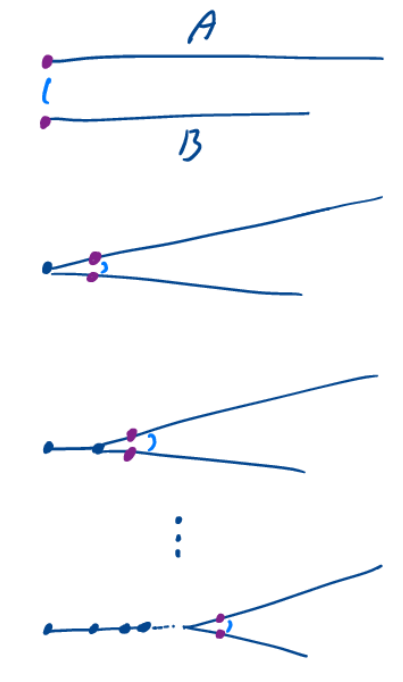
\includegraphics[width = 2.80cm]{immagini/ordine_totale_buoni_ordini.png}
\end{wrapfigure}

\textcolor{MidnightBlue}{\underline{Idea}: Il corollario ci dice che vale al più una delle alternative, quindi la difficoltà risiede nel dimostrare che una si verifica. Molto vagamente potremmo ragionare così.
Identifichiamo, progressivamente, segmenti iniziali sempre più lunghi di $A$ e $B$. All'inizio identifichiamo il minimo di $A$ con il minimo di $B$, poi il secondo elemento di $A$ con il secondo elemento di $B$, etc. Fatti $\omega$
passaggi avremo identificato un segmento iniziale di $A$, diciamo $A_x$, isomorfo a $\omega$, con un $B_y$, anch'esso ovviamente isomorfo a $\omega$. Bene: continuiamo identificando $x$ con $y$. Quando potrebbe bloccarsi il procedimento?
Solo se, ad un certo punto, abbiamo identificato interamente uno dei due insiemi, con un segmento iniziale dell'altro - perché altrimenti, abbiamo identificato due segmenti iniziali $A_x$ e $B_y$ e possiamo continuare attaccando $x$ a $y$. È 
come la chiusura di una cerniera lampo : ad ogni istante c'è un prossimo dente.\\
\textcolor{red}{Questa discorso, però, non è una dimostrazione.} Se vogliamo, sarebbe un tentativo di costruire l'isomorfismo cercato per \textcolor{purple}{ricorsione transfinita}. Il guaio è che i numeri che permetterebbero di numerare i passaggi della costruzione,
gli \textcolor{purple}{ordinali}, sono appunto l'oggetto che stiamo tentando di costruire.}

\begin{proof}
	Per il corollario visto prima, si può verificare al più una delle tre condizioni, altrimenti avremmo un assurdo, verifichiamo dunque che se ne verifichi almeno una. Consideriamo $f$ definita come segue:
	\[ f = \{(a,b) \in A \times B | A_a \sim B_b\}
		\]
	Vogliamo dimostrare che $f$ è una funzione crescente, che $\Dom(f)$ è un segmento iniziale di $A$, e che $\Imm(f)$ è un segmento iniziale di $B$, da cui $f$ manda segmenti iniziali in segmenti iniziali. Quindi $f$ è un isomorfismo fra un segmento iniziale di $A$ e uno di $B$.
	Infine dimostriamo che necessariamente $\Dom(f) = A$ o $\Imm(f) = B$, e questo conclude la dimostrazione perché se si verifica una delle due o tutte e due, abbiamo ottenuto la tesi del teorema. Procediamo ora con tutte le verifiche.
	\begin{itemize}
		\item[$\boxed{\text{$f$ è una funzione}}$] \textcolor{MidnightBlue}{Supponiamo per assurdo $(a,b) \in f$ e $(a,b') \in f$ con $b \ne b'$. Senza perdita di generalità supponiamo $b < b'$ (quindi $B_b$ s.i. proprio di $B_{b'}$), e, per la definizione data di $f$ ciò corrisponde a:
		\[ B_b \sim A_a \sim B_{b'}
			\]
		dunque $B_{b'}$ sarebbe isomorfo al suo segmento iniziale proprio $B_b$ $\lightning$.}
		\item[$\boxed{\text{$f$ è crescente}}$] \textcolor{MidnightBlue}{Dati $a,a' \in A$, con $a<a'$, dobbiamo dimostrare $f(a) < f(a')$. Supponiamo, per assurdo $f(a') \leq f(a)$, abbiamo allora:
		\[ A_{a'} \sim B_{f(a')} \preceq B_{f(a)} \sim A_a
			\]
		dove i due isomorfismi, vengono semplicemente dalla definizione di $f$, e $B_{f(a')} \preceq B_{f(a)}$ segue da $B_{f(a')} \subseteq B_{f(a)}$, che vale perché stiamo supponendo $f(a') \leq f(a)$ per ipotesi assurda.
		Abbiamo quindi ottenuto che $A_{a'}\preceq A_a$, ovvero $A_{a'}\subseteq A_a \implies a' \leq a$, che è assurdo perché avevamo per ipotesi $a < a'$.}
		\item[$\boxed{\text{$\Dom(f)$ è s.i. di $A$}}$] \textcolor{MidnightBlue}{Sia $a \in \Dom(f)$ e $a' < a$, vogliamo dimostrare che $a' \in \Dom(f)$. L'ipotesi $a \in \Dom(f)$ equivale a dire che $A_a \sim B_b$, per qualche $b \in B$,
		inoltre, essendo $a' < a$ si ha $A_{a'} \subsetneq A_a \to A_{a'} \prec A_a$, per cui $A_{a'} \prec B_b$. A questo punto esiste $b' \in B_b \subsetneq B$ tale che $A_{a'} \sim (B_{b})_{b'}$, per definizione di $\prec$, e, osservando che $(B_b)_{b'} = B_{b'}$,
		si ha proprio $A_{a'} \sim B_{b'} \implies (a',b') \in f$, per cui $a' \in \Dom(f)$.}
		\item[$\boxed{\text{$\Imm(f)$ è s.i. di $B$}}$] \textcolor{MidnightBlue}{Dimostrazione simmetrica alla precedente.}
		\item[$\boxed{\begin{aligned}\text{$\Dom(f) = A$} \\ \text{o $\Imm(f) = B$}\end{aligned}}$] \textcolor{MidnightBlue}{Se così non fosse, per la terza e quarta verifica, avremmo contemporaneamente $\Dom(f) = A_a$ e $\Imm(f) = B_b$ \footnote{Stiamo negando un OR quindi l'unica possibilità è che siano entrambe false.},
		per opportuni $a \in A$ e $b \in B$. Per la seconda verifica $f$ è crescente, quindi è un isomorfismo fra $\Dom(f) = A_a$ e $\Imm(f) = B_b$, pertanto,
		si ottiene proprio $A_a \sim B_b$, e quindi, per definizione di $f$, $(a,b) \in f$, da cui $a \in \Dom(f) = A_a \; \lightning$ (oppure $b \in \Imm(f) = B_b \; \lightning$). Segue quindi che almeno una delle due condizioni è sempre vera.}
	\end{itemize}
\end{proof}

\begin{exercise}[Sottoinsiemi propri e buoni ordinamenti]
	Sia $(A,<)$ un buon ordine e sia $B \subsetneq A$. Dimostra che $B \preceq A$, ma non necessariamente $B \prec A$.
\end{exercise}

\begin{soln}
	In primis osserviamo che non può valere $A \prec B$, infatti, se $A$ fosse isomorfo ad un segmento iniziale proprio di $B$, sia $B_b$, per $b \in B$,
	allora $b \leq f(b)\footnote{Notare che la disuguaglianza continua a valere solo perché $B \subseteq A$, in generale se i buoni ordinamenti sono diversi non vale.} \in B_b \implies b \leq f(b) < b \; \lightning$. Per il teorema appena dimostrato sappiamo che la classe dei buoni ordini è totalmente ordinata, per cui vale necessariamente $B \preceq A$.\\
	Per avere un controesempio di $B \subsetneq A \notimplies B \prec A$ ci basta considerare $(\omega,<)$ e il sottoinsieme proprio $2\omega$ dei numeri pari, in questo caso infatti abbiamo $(2\omega,<_{|2\omega}) \sim (\omega,<)$,
	che è dato dalla funzione che mappa $i \mapsto n_i$ (l'$i$-esimo numero pari preso in ordine strettamente crescente).
\end{soln}

\begin{exercise}[Unione di buoni ordinamenti]
	Sia $(A,<_A)$ un ordine totale con $A = \bigcup S$. Supponiamo che:
	\begin{enumerate}[1.]
		\item ogni $X \in S$ è un buon ordine con la restrizione $<_{A|X}$
		\item per ogni $X,Y \in S$, o $X$ è segmento iniziale di $Y$ o $Y$ è segmento iniziale di $X$
	\end{enumerate}
	Dimostra che allora $(A,<_A)$ è un buon ordine. Esibisci inoltre un controesempio alla tesi eliminando la condizione 2 dalle ipotesi.
\end{exercise}

\begin{soln}
	Dato $B \subseteq A$ diverso dal vuoto, allora, detto $Z = \{X \in S | X \cap B \ne \emptyset\}$, possiamo considerare $\bigcap Z$ ed osservare che $\bigcap Z = X \in Z$, infatti,
	se per assurdo ci fosse almeno un elemento di un altro insieme, $y \in \bigcap Z$, con $y \in Y \in S \land y \not \in X$, allora, essendo che per ipotesi o $X$ è segmento iniziale di $Y$ o viceversa, si ha: nel primo caso $y$ non può stare nell'intersezione perché non appartiene ad $X$, per cui abbiamo un assurdo,
	nel secondo - se $Y$ segmento iniziale di $X$ - avremmo che $y \in X$ e quindi ancora un assurdo.\\
	Abbiamo quindi che $\emptyset \ne \bigcap Z = X \in Z$, per cui $X \cap B \ne \emptyset$, ed è ben definito $b = \min_{<_{A|X}} (X \cap B) = \min_{<_{A|X}} \left(\bigcap Z \cap B\right)$.\\
	Non resta che osservare che $b$ è il minimo anche per gli elementi di $B \setminus X$. Dato $b' \in B \setminus X$, allora $b' \in Y \in Z$, con $Y \ne X$, osserviamo ora che $X$ è segmento iniziale di $Y$ (deve valere una delle due cose per ipotesi, ed essendo $X = \bigcap Z \subseteq Y$, siamo necessariamente in questo caso),
	per cui $X = Y_c$ (siamo in un buon ordinamento), per qualche $c \in Y$, e in particolare si ha proprio $b < c \leq b'$, infatti la prima disuguaglianza è banale, mentre la seconda deriva dal fatto che $b' \in B \setminus X$ 
	e per la proprietà dei segmenti iniziali se fosse $b' < c$ allora $b' \in Y_c = X$ che è assurdo.\\
	Per il controesempio alla tesi nel caso in cui manchi la seconda condizione, consideriamo l'insieme $\QQ = \{q_n | n \in \omega\}$ di cui abbiamo fissato un'enumerazione, detto $Q_n = \{q_i | i < n\}$, naturalmente si ha:
	\[ \QQ = \bigcup_{n \in \omega} Q_n
		\]
	dove $(\QQ,<)$ è totalmente ordinato e i $(Q_n,<_{|Q_n})$ sono bene ordinati dalla restrizione dell'ordinamento di $\QQ$ essendo insiemi finiti, inoltre non è vero che presi $Q_n$ e $Q_m$ uno non è necessariamente segmento iniziale dell'altro,
	perché nell'enumerazione possiamo (e necessariamente dovrà accadere) aggiungere anche elementi più piccoli. Siamo pertanto nelle condizioni dell'esercizio tranne che per 2., e quindi naturalmente non si ottiene che $(\QQ,<)$ è bene ordinato.
\end{soln}

\subsection{Operazioni aritmetiche fra buoni ordinamenti}
Per ora, non abbiamo visto molti esempi di buoni ordini. Le operazione definite in questa sezione forniscono una prima sorgente di esempi concreti.
Nel seguito del corso, vedremo buoni ordini assai più versatile di quelli ottenibili con queste operazioni.

\begin{definition}[Somma di ordini totali]
	Dati $(A,<_A)$ e $(B,<_B)$ ordini totali. Definiamo la \vocab{somma di ordini totali} come:
	\[ (A,<_A) + (B,<_B) \Mydef (A \sqcup B, <_+)
		\]
	dove, ricordiamo che $A \sqcup B = (A \times\{0\}) \cup (B \times \{1\})$, e $<_+$ è definito da:
	\[ \begin{split}
		(x,y) <_+ (x',y') &\Mydef (y = 0 \land y' = 1) \\
						  &\lor (y = 0 \land y' = 0 \land x <_A x') \\
						  &\lor (y = 1 \land y' = 1 \land x <_B x')
	\end{split}
		\]
\end{definition}

\textcolor{MidnightBlue}{L'idea è che $(A,<_A) + (B,<_B)$ si ottiene attaccando $(B,<_B)$ in coda a $(A,<_A)$}.

\begin{figure}[H]
	\centering
	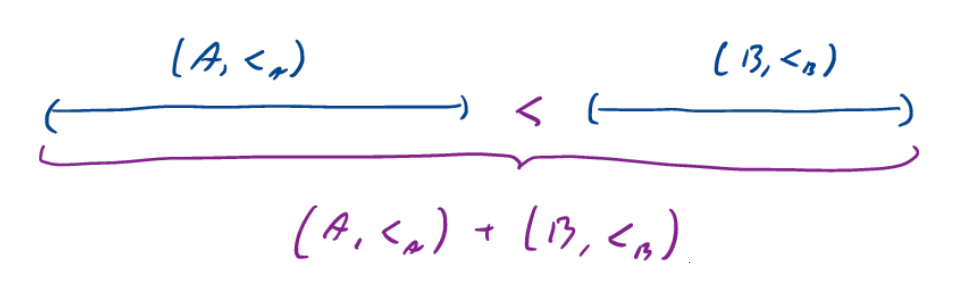
\includegraphics[width = 7.5cm]{immagini/somma_ordini_totali.png}
\end{figure}

Riproponiamo, per completezza, la definizione di prodotto lessicografico.

\begin{definition}[Prodotto di lessicografico]
	Siano $(A,<_A)$ e $(B,<_B)$ ordini totali. Definiamo il \vocab{prodotto del lessicografico}:
	\[ (A,<_A) \cdot (B,<_B) \Mydef (A \times B, <_\times)
		\]
	dove $<_\times$ è definito da:
	\[ (x,y) <_\times (x',y') \Mydef (y <_B y') \lor (y = y' \land x <_A x')
		\]
\end{definition}

\textcolor{MidnightBlue}{L'idea di confrontare prima la seconda componente, deriva dal fatto che $(A,<_A) \cdot (B,<_B)$ sono 
tante copie di $(A,<_A)$ giustapposte, quanti sono gli elementi di $B$ (e quindi associate nello stesso ordine)}.

\begin{figure}[H]
	\centering
	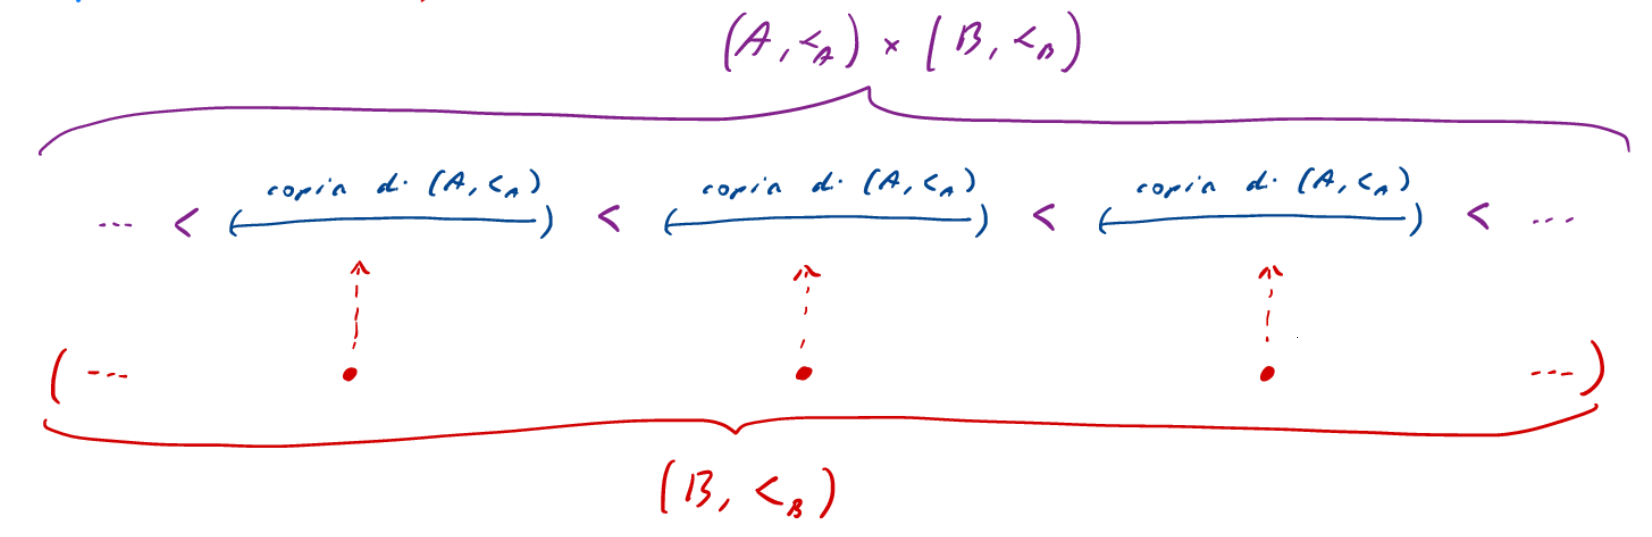
\includegraphics[width = 10.5cm]{immagini/ordine_lessicografico.png}
\end{figure}

Per definire l'esponenziale ci serve la nozione di supporto.

\begin{definition}[Supporto di una funzione da un insieme a un buon ordine]
	Dato un buon ordine $(B,<)$ e $f : A \rightarrow B$, il \vocab{supporto} di $f$ è:
	\[ \supp_B(f) \Mydef \{x \in A | f(x) \ne \min_{<_B} B\}
		\]
	(ometteremo il pedice $B$ quando è chiaro cosa sia $B$).
\end{definition}

\textcolor{MidnightBlue}{Il supporto è quindi il sottoinsieme dei punti sull'insieme di partenza, sui quali $f$ non assume il minimo del buon ordinamento in arrivo quest'ultimo.}

\begin{definition}[Esponenziali di ordini totali]
	Dati $(A,<_A)$ e $(B,<_B)$ ordini totali, definiamo l'\vocab{esponenziale di ordini totali}:
	\[ (A,<_A)^{(B,<_B)} \Mydef (\{f \in {}^{B}A \, : \, |\supp_A f| < \aleph_0\},<_{\exp})
		\]
	dove l'insieme è quello delle funzioni a supporto finito (quindi che su un numero finito di punti non assumono il valore $\min_{<_B}B$), e l'ordine $<_{\exp}$ è definito da:
	\[ f <_{\exp} g \Mydef (f \ne g) \land (f(m) <_A g(m))
		 \]
	dove $m$ è il massimo valore in $B$ su cui $f$ e $g$ sono diverse, cioè non sono entrambe $\min A$, $m := \max_{<_B}\{x \in B | f(x) \ne g(x)\}$.
\end{definition}

\textcolor{MidnightBlue}{L'idea è che una funzione $B \rightarrow A$ può essere vista come una specie di tupla con tante componenti quanti sono gli elementi di $B$\footnote{D'altronde abbiamo visto che $|{}^{B}A| = |A|^{|B|}$, il che ci fa notare che la definizione data di insieme di funzioni come una sorta di esponenziazione di un insieme ad un altro, è coerente con quella di esponenziazione come prodotto cartesiano ripetuto un numero di volte pari alla cardinalità dell'esponente, da qui l'identificazione di ${}^{B}A$ con $\underbrace{A \times \ldots \times A}_{\text{$|B|$ volte}}$, che ci dà l'intuizione descritta (e che formalmente si traduce nell'insieme di funzioni, che sarà poi la vera definizione di prodotto cartesiano).}.
Ordinare queste tuple lessicograficamente significa (generalizzando l'idea usata per il prodotto lessicografico) che vince la componente diversa più a destra, e se definitivamente c'è il minimo in entrambe le tuple, per la finitezza del supporto, basta confrontare l'ultima componente dove sono diverse, ossia la componente corrispondente all'elemento di $B$ più grande su cui le funzioni sono diverse.}

\begin{exercise}
	Verificare che $(\omega,<)^{(\omega,<)} \sim (\NN[x],\prec)$, dove $\NN[x]$ denota l'insieme dei polinomi a coefficienti in $\NN$, e definiamo:
	\[ p \prec q \Mydef \exists N \in \NN \; \forall x \in \NN \; x > N \rightarrow p(x) < q(x)
		\]
	ossia $p \prec q$ se $p(x)<q(x)$ definitivamente.
\end{exercise}

\begin{soln}
	Possiamo scrivere esplicitamente l'isomorfismo come segue:
	\[ (\omega,<)^{(\omega,<)} \to (\NN[x],\prec) : f \mapsto \sum_{i = 0}^{\infty}f(i)x^i
		\]
	osserviamo in primis che la sommatoria è in realtà una somma di un numero finito di termini in quanto $f$ ha supporto finito,
	dunque ciò che otteniamo è un polinomio e quindi la mappa è ben definita. Si vede facilmente che è surgettiva, infatti, dato $p(x) = \sum_{i = 0}^n a_i x^i$, 
	è sufficiente considerare:
	\[ f : \omega \to \omega : i \mapsto \begin{cases}
		a_i &\text{se $0 \leq i \leq n$} \\
		0 &\text{altrimenti}
	\end{cases}
		\] 
	che è naturalmente una funzione a supporto finito dai naturali ai naturali. Infine, verifichiamo la stretta crescenza, date $f < g$, abbiamo $f(m) < g(m)$, 
	per $m$ massimo valore in $\omega$ per cui sono distinte; si danno due casi, o $f(m) = 0$ e quindi $g(m) > 0$, in questo caso a $g$ corrisponde un polinomio $q(x)$ di grado 
	più grande strettamente, dunque, se $f$ corrisponde a $p(x)$, si ha $q(x) = \text o(p(x))$ per $x \to +\infty$, per cui $\lim_{x \to +\infty} \frac{q(x)}{p(x)} = +\infty$, che equivale alla definizione data di $p \prec q$.
	Nel caso in cui $f(m) > 0$, allora $p(x)$ e $q(x)$ sono polinomi dello stesso grado, ma $q(x)$ ha coefficiente di testa maggiore strettamente di quello di $p(x)$,
	per cui $\lim_{x \to +\infty} \frac{q(x)}{p(x)} > 0 \implies p \prec q$.
\end{soln}

\begin{proposition}[Somma, prodotto ed esponenziale di buoni ordini è un buon ordine]
	Se $(A,<_A)$ e $(B,<_B)$ sono buoni ordini, allora anche:
	\[ (A,<_A) + (B,<_B) \qquad (A,<_A) \cdot (B,<_B) \qquad (A,<_A)^{(B,<_B)}
		\]
	sono buoni ordini.
\end{proposition}

\begin{proof}
	Si tratta di banali verifiche, \textcolor{red}{eccetto la terza}.\\
	La relazione $<_{\exp}$ è irriflessiva per definizione richiede $f \ne g$, dunque se sono uguali non sono in relazione. Occorre quindi verificare la transitività.
	Assumiamo $f <_{\exp} g$ e $g <_{\exp} h$, dove naturalmente $f,g,h \in {}^B A$, e poniamo:
	\begin{align*}
		&m_1 = \max_{<_B}\{x\in B | f(x) \ne g(x)\} \\
		&m_2 = \max_{<_B}\{x\in B | g(x) \ne h(x)\} \\
		&m_3 = \max_{<_B}\{x\in B | f(x) \ne h(x)\}
	\end{align*}
	detto $m := \max(m_1,m_2)$, abbiamo $f(m) \leq_A g(m) \leq_A h(m)$, dove la prima disuguaglianza è stretta se $m = m_1$, e la seconda lo è se $m = m_2$, in ogni caso, almeno una delle due disuguaglianze è sempre stretta per cui abbiamo $f(m) <_A h(m)$.
	Osserviamo inoltre che se $x > m$ allora necessariamente $f(x) = g(x) = h(x)$ perché avremmo in questo caso che $x > m_1,m_2$, che sono i massimi su cui si hanno le disuguaglianze, per cui $m = m_3$.\\
	Mostriamo ora che $<_{\exp}$ è un ordine totale, se $f \ne g$ allora è ben definito $m := \max_{<_B}\{x \in B | f(x) \ne g(x)\}$, infatti le funzioni sono a supporto finito per ipotesi dunque stiamo prendendo il massimo su un insieme finito e 
	non vuoto essendo le funzioni diverse, si conclude per la totalità di $<_A$ che vale necessariamente o $f(m)<_A g(m)$ o $g(m) <_A f(m)$, nel primo caso $f <_{\exp} g$, nel secondo $g <_{\exp} f$.\\
	Resta da verificare che l'ordine ottenuto esponenziando è buono. Chiamiamo $S$ l'insieme delle funzioni a supporto finito da $B$ ad $A$ e supponiamo per assurdo che non sia bene ordinato, cioè:
	\[ \underbrace{\exists f \in S \; \exists A \subseteq S (f \in A}_{\text{c'è un $A \subseteq S$ non vuoto}}\land\underbrace{\forall g \in A \; \exists h \in A \; h <_{\exp} g}_{\text{che non ha minimo}})
		\]
	Da quanto appena scritto possiamo fissare una $f \in S$ tale che $\exists A \subseteq S$ etc. con queste proprietà:
	che il massimo del suo supporto sia il minimo possibile, $m:=\max_{<_B}(\supp_A(f))$, e che, a parità di $m$, il valore di $f(m)$ sia minimo.
	Fissata $f$ come scritto, possiamo fissare ora anche $A$ nella formula in modo tale che $f \in A$ ed $A$ sia un sottoinsieme senza minimo.
	Il nostro obiettivo ora è costruire $\widetilde{A} \subseteq S$ che non abbia minimo e contenga una funzione $\widetilde{f}$ con $\widetilde{m} := \max_{<_B}(\supp_A(f)) <_B m$, in questo modo neghiamo la minimalità di $m$ ed otteniamo la contraddizione voluta.
	Osserviamo innanzitutto che $A$ può essere ripartito in generale come:
	\begin{align*}
		&A_1 = \{g \in A |\max_{<_B}(\supp_A(g)) <_B m\} \\
		&A_2 = \{g \in A |\max_{<_B}(\supp_A(g)) = m \land g(m) = f(m)\} \\
		&A_3 = \{g \in A |\max_{<_B}(\supp_A(g)) = m \land f(m) <_A g(m)\} \\
		&A_4 = \{g \in A |m <_B \max_{<_B}(\supp_A(g))\}
	\end{align*}
	e segue dalla definizione che le funzioni in $A_1$, sono $<_{\exp}$ di quelle in $A_2$, che sono $<_{\exp}$ etc. fino ad $A_4$ - è sufficiente pensare alle definizioni che abbiamo dato -.
	Però $A_1$ è vuoto, perché altrimenti, presa $f' \in A_1$, abbiamo $f' \in A$ e $\max(\supp_A(f))<m$ contro la minimalità di $m$.
	Abbiamo invece che $A_2$ non è vuoto perché contiene $f$, e non ha minimo, infatti, se avesse minimo, questo dovrebbe essere anche minimo di $A$ - per la minimalità di $m$, avremmo preso la $f$ che fa meno su $m$ e quindi necessariamente la più piccola di tutte -, che non ha minimo per ipotesi.\\
	Concentriamoci ora su $A_2$. Tutte le $g \in A_2$ assumono il medesimo valore su $m$, quindi, comparando due di queste funzioni con $<_{\exp}$, il valore assunto da entrambe su $m$ 
	è irrilevante perché $<_{\exp}$ confronta la massima componente in cui sono diverse, per cui la funzione:
	\[ H : A_2 \rightarrow S : g \mapsto \widehat{g} \quad\text{con}\quad\widehat{g}(x) = \begin{cases}
		\min A &\text{se $x = m$}\\
		g(x) &\text{altrimenti}
	\end{cases}
		\]
	è strettamente crescente, poiché dove le funzioni sono uguali poniamo semplicemente il loro valore uguale a $\min A$, cosa ininfluente per $<_{\exp}$, mentre dove vale la disuguaglianza continua a valere nell'immagine poiché 
	non modifichiamo nulla in tal caso. Per cui $\widetilde{A} := H[A_2]$ non ha minimo, altrimenti, essendo $H$ strettamente crescente, tornando indietro anche $A$ lo avrebbe.
	Ora, però, segue dalla definizione di $H$, che, fissata $g \in A_2$, $\supp(\widehat{g}) = \supp(g) \setminus \{m\}$ (lo abbiamo rimosso ``a mano'' con $H$), quindi, ponendo $\widetilde{f} := \widehat{g}$, abbiamo $\max(\supp(\widehat{f}))<m$ (prima $m$ era il massimo valore del supporto e non dava $\min A$, ora 
	che l'abbiamo rimosso dal supporto, avendolo preso come il max del precedente supporto, ciò che rimane è necessariamente strettamente minore), e questo contraddice la minimalità di $m$.\footnote{Cose che andrebbero verificate per rendere precisa questa dimostrazione: perché posso fissare $A$ e $f$ tali che..., in altre parole perché esistono $A$ ed $f$ tali per cui...; perché 
	si può partizionare $A$ in quei 4 insiemi; fare le verifiche delle disuguaglianze tra gli elementi dei 4 insiemi; precisare meglio i dettagli della parte finale.}
\end{proof}

\begin{proposition}[Buona definizione delle operazioni tra ``classi di isomorfismo'']
	Le operazioni aritmetiche sui buoni ordini \vocab{passano al quoziente modulo isomorfismi}. Ossia, dati due buoni ordinamenti $\mathcal A = (B,<_A)$
	e $\mathcal B = (B,<_B)$, e dati $\mathcal A' = (A',<_{A'}) \sim \mathcal A$ e $\mathcal{B}' = (B',<_{B'}) \sim \mathcal B$, si ha:
	\[ \mathcal{A} + \mathcal{B} \sim \mathcal{A}' + \mathcal{B'} \qquad \mathcal{A} \cdot \mathcal{B} \sim \mathcal{A}' \cdot \mathcal{B'} \qquad \mathcal{A}^{\mathcal{B}} \sim \mathcal{A}'^{\mathcal{B'}}
		\]
	quindi le operazioni fra buoni ordini sono equivalenti modulo l'essere isomorfi.\footnote{In altre parole le operazioni tra buoni ordini sono definite sulle classi di equivalenza di buoni ordini isomorfi, e la proposizione mostra che queste 
	operazioni sono ben definite.}
\end{proposition}

\begin{proof}
	Fissati gli isomorfismi $f : A \rightarrow A'$ e $g : B \rightarrow B'$, è facile scrivere esplicitamente gli isomorfismi richiesti. Per esempio, nel caso di $\mathcal{A}^{\mathcal{B}}$, si considera la restrizione alle funzioni a supporto finito di:
	\[ {}^{B}A \rightarrow {}^{B'}A' : h \mapsto f \circ h \circ g^{-1}
		\]
	in altre parole, l'isomorfismo richiesto per dimostrare la tesi, che è quello scritto sopra, è quello che manda $h$ nella mappa che fa commutare il seguente diagramma:
	\[\begin{tikzcd}
		B & A \\
		{B'} & {A'}
		\arrow["h", from=1-1, to=1-2]
		\arrow["{g^{-1}}", from=2-1, to=1-1]
		\arrow[from=2-1, to=2-2]
		\arrow["f", from=1-2, to=2-2]
	\end{tikzcd}\]
	andrebbe verificato che anche la nuova funzione $f \circ h \circ g^{-1}$ sia a supporto finito, ma questo segue dal fatto che $f$ e $g$ sono isomorfismi di ordini,
	in particolare vale che $g^{-1}[\supp_{A'}(f \circ h \circ g^{-1})] = \supp_A(h)$ (va verificato il doppio contenimento e può essere fatto facilmente tenendo conto e seguendo il diagramma sopra),
	da cui la bigezione e quindi la finitezza di $\supp_{A'}(f \circ h \circ g^{-1})$.
\end{proof}

\begin{exercise}[Buona definizione delle operazioni tra buoni ordini]
	Fare le altre verifiche della proposizione sopra.
\end{exercise}

\begin{proposition}[Proprietà delle operazioni sui buoni ordini]
	Siano $\mathcal{A} = (A,<_A)$, $\mathcal{B} = (B,<_B)$ e $\mathcal{C} = (C,<_C)$ buoni ordini. Allora:\footnote{Valgono in realtà anche l'esistenza e le proprietà degli elementi neutri per $\cdot$ e $+$.}
	\[\begin{split}
		\text{\textcolor{red}{associatività:}} &\quad (\mathcal A + \mathcal B) + \mathcal C \sim \mathcal A + (\mathcal B + \mathcal C) \quad (\mathcal A \cdot \mathcal B) \cdot \mathcal C \sim \mathcal A \cdot (\mathcal B \cdot \mathcal C)\\
		\text{\textcolor{red}{distributività a sinistra:}} &\quad  \mathcal A \cdot (\mathcal B + \mathcal C) \sim \mathcal A \cdot \mathcal B + \mathcal A \cdot \mathcal C \\
		\text{\textcolor{red}{proprietà delle potenze:}} &\quad {\mathcal A}^{\mathcal B + \mathcal C} \sim \mathcal A^{\mathcal B} \cdot {\mathcal A}^{\mathcal C} \qquad ({\mathcal A}^{\mathcal B})^{\mathcal{C}} \sim {\mathcal A}^{\mathcal B \cdot \mathcal C}
	\end{split}\]
\end{proposition}

\begin{proof}
	Facili verifiche.
\end{proof}

\begin{exercise}[Proprietà delle operazioni tra buoni ordini]
	Fare qualcuna delle verifiche delle proprietà sopra.
\end{exercise}

\textcolor{red}{Non} tutte le proprietà delle operazioni aritmetiche su $\omega$ valgono per i buoni ordini.

\begin{exercise}[Proprietà \textcolor{red}{false} delle operazioni tra buoni ordini]
	Esibire controesempi alle seguenti:
	\textcolor{red}{\begin{align*}
		& \mathcal A + \mathcal B \sim \mathcal B + \mathcal A &(\mathcal A + \mathcal B) \cdot \mathcal C \sim \mathcal A \cdot \mathcal C + \mathcal B \cdot \mathcal C \\
		& \mathcal A \cdot \mathcal B \sim \mathcal B \cdot \mathcal A &(\mathcal A \cdot \mathcal B)^{\mathcal C} \sim \mathcal A^{\mathcal C} \cdot \mathcal B^{\mathcal C}
	\end{align*}}
	ovvero non valgono: \textcolor{red}{commutatività}, \textcolor{red}{distributività a destra} e \textcolor{red}{potenza di un prodotto}.
\end{exercise}

\begin{soln}
	Vediamo controesempi caso per caso.
	\begin{itemize}
		\item[\textcolor{red}{$\boxed{\text{commutatività $+$}}$}] Basta considerare $1+\omega$ e $\omega + 1$ (sia $1$ che $\omega$ sono buoni ordini), infatti abbiamo che:
		\begin{align*}
			1+\omega = (1 \sqcup \omega, <_+) \qquad \omega + 1 = (\omega \sqcup 1, <_+) 
		\end{align*}
		dove $1 \sqcup \omega = (1,0)\cup (\omega \times \{1\}) = \{(1,0),(0,1),(1,1),(2,1),\ldots\}$, con $<_+$ che è l'ordine dato dalla somma di buoni ordini, dunque $(1,0)<_+(n,1)$, $\forall n \in \omega$. Si vede facilmente
		quindi che $1 + \omega$ (oltre ad essere un buon ordine in quanto somma di buoni ordini) è superiormente illimitato e vale il principio del massimo, dunque $1+\omega \sim \omega$. Viceversa, dove $\omega \sqcup 1 = (\omega \times \{0\})\cup \{(1,1)\} = \{(1,1),(0,0),(1,0),(2,0),\ldots\}$,
		con $<_+$ che è sempre l'ordine dato dalla somma di buoni ordini, ma in questo caso si ha $(n,0) <_+ (1,1)$, $\forall n \in \omega$, dunque $\omega + 1$ è superiormente limitato, pertanto non può essere isomorfo ad $\omega$, dunque $1 + \omega \ne \omega + 1$.
		\item[\textcolor{red}{$\boxed{\text{commutatività $\cdot$}}$}] È sufficiente considerare $2 \cdot \omega$ e $\omega \cdot 2$, infatti in questo caso i buoni ordinamenti sono:
		\[ (2 \times \omega,<_\times) \qquad (\omega \times 2, <_\times)
			\]
		Si osserva che $(2 \times \omega,<_\times) \sim (\omega,<)$, infatti, detto $n_i$ l'$i$-esimo numero pari e $m_i = n_i+1$ l'$i$-esimo numero dispari, la mappa $(0,i) \mapsto n_i$ e $(1,i) \mapsto m_i$ è l'isomorfismo cercato. D'altra parte, per le proprietà sopra, si ha $\omega \cdot 2 = \omega \cdot (1 + 1) = \omega + \omega$,
		e non si può avere isomorfismo in quanto $\omega$ è naturalmente isomorfo al segmento iniziale proprio $(\omega,<) \prec \omega + \omega = (\omega \sqcup \omega, <_+)$.
	\end{itemize}
\end{soln}

Un altro tranello in cui si potrebbe cadere è credere che le operazioni sui buoni ordini generalizzino quelle sulle cardinalità. Questo è vero per le cardinalità finite, dove le operazioni di $\omega$ coincidono con quelle cardinali e ordinali, e anche in generale 
per somma e prodotto - come è ovvio dalla definizione - ma fallisce per l'esponenziazione quando consideriamo buoni ordinamenti infiniti.

\begin{exercise}[Cardinalità dell'esponenziazione ordinale]
	Dimostra che se $\mathcal A = (A,<_A)$ e $\mathcal B = (B,<_B)$ sono buoni ordini con $|A| = |B| = \aleph_0$ e $(C,<_C) = \mathcal A^{\mathcal B}$ allora $|C| = \aleph_0$.\footnote{\underline{\textbf{Hint}}: ricordare che $\psf(\omega) = \aleph_0$ e pensare a come si possa identificare ciò con $\omega^\omega$.}
\end{exercise}

\begin{soln}
	A meno di bigezioni, vogliamo dimostrare che $|\omega^\omega| = \aleph_0$, per fare ciò osserviamo che data $f \in \omega^\omega$, essa è a supporto finito, quindi come insieme la si può identificare univocamente come un insieme finito - cioè lasciando solo le coppie corrispondenti 
	a elementi che non danno $\min \omega = 0$ tramite $f$ - per cui si ha che $\{f \in \omega^\omega : |\supp_\omega(f)| < \aleph_0\} \hookrightarrow \psf(\omega \times \omega) : f \mapsto f_{|\supp_\omega(f)}$ è ben definita, e iniettiva (per tornare indietro basta estendere il dominio a tutto $\omega$ ed associare ai nuovi elementi 0).
	Abbiamo quindi $|\omega^\omega| \leq \aleph_0$. Viceversa è ovvio che $\omega \hookrightarrow \omega^\omega : n \mapsto f_n$, ovvero la funzione tale che $f_n(n) = 1$ e $f_n(m) = 0$, per ogni $m \in \omega\setminus\{n\}$, che è ovviamente a supporto finito, per cui abbiamo facilmente l'iniettività e quindi la disuguaglianza dal basso.
\end{soln}

\newpage

\subsection{Gli ordinali di Von Neumann}
In questa sezione definiremo gli ordinali di Von Neumann. L'idea che vogliamo concretizzare è che, siccome abbiamo visto che, 
a meno di isomorfismi, due buoni ordinamenti sono sempre l'uno nell'altro, unendo fra loro tutti i buoni ordinamenti - o tutte le classe di isomorfismo 
di questi - dovrebbe potersi costruire un buon ordinamento più grande di tutti. Questa vasta struttura sarà inevitabilmente una classe propria:
la classe dei \vocab{numeri ordinali}, i cui elementi sono rappresentanti di tutte le possibili classi di isomorfismo di buoni ordini.

\begin{definition}[Insieme transitivo]
	L'insieme $\alpha$ è \vocab{transitivo} se $\forall x \in \alpha \; x \subseteq \alpha$, o equivalentemente, se $\forall x \in \alpha \, \forall y \in x \; y \in \alpha$ (da cui il termine transitivo).
\end{definition}

\textcolor{MidnightBlue}{Ossia: diciamo che $\alpha$ è transitivo se gli elementi degli elementi di $\alpha$ sono, a loro volta, elementi di $\alpha$, cioè se gli elementi sono a loro volta sottoinsiemi dell'insieme insieme (si pensi ad esempio a $\omega$).}

\begin{definition}[Ordinali di Von Neumann]
	L'insieme $\alpha$ è un \vocab{ordinale} se è \textcolor{red}{transitivo e bene ordinato dalla relazione di appartenenza}. Formalmente, l'insieme transitivo $\alpha$
	è un ordinale se $(\alpha, <_\alpha)$ è un buon ordine, con:
	\[ <_\alpha \Mydef \{(x,y) \in \alpha \times \alpha | x \in y\}\,\footnote{Esattamente come accade su $\omega$: $x < y \leftrightarrow x \in y \leftrightarrow (x,y) \in <$.}
		\]
	Denotiamo con \vocab{$\Ord$} la classe degli ordinali\footnote{Tale classe contiene un elemento per ciascun buon ordinamento, ad esempio, preso $(\omega,<)$, come rappresentante della sua classe
	di isomorfismo, prendiamo $\omega$ stesso - inteso come buon ordinamento transitivo e ordinato dall'appartenenza - come rappresentante della ``classe di equivalenza'' nella classe dei buoni ordini (attenzione a non confondere i due significati del termine classe).}, per cui:
	\[ \alpha \in \Ord \Mydef \; \text{``$\alpha$ è transitivo e ben ordinato da $\in$''}
		\]
\end{definition}

\begin{example}[Esempi di ordinali]
	Alcuni esempi di ordinali già incontrati:
	\begin{itemize}
		\item $\omega$ è un ordinale
		\item gli elementi di $\omega$ sono ordinali
		\item $s(\omega) = \omega \cup \{\omega\}$ è un ordinale
	\end{itemize}
\end{example}

\begin{remark}[$\Ord$ è una classe transitiva]
	\label{Ord_trans}
	Se $\alpha \in \Ord$ e $\beta \in \alpha$, allora $\beta \in \Ord$ e $\beta = \alpha_\beta$, ovvero $\beta$ è un ordinale ed è il segmento iniziale principale di $\alpha$, determinato da $\beta$.
	In particolare la classe degli ordinali $\Ord$ è transitiva.\footnote{Cioè tutti gli ordinali sono a loro volta insiemi di ordinali di più piccoli.}
\end{remark}

\begin{proof}
	Siccome $\beta \in \alpha$, per la transitività di $\alpha$, $\beta \subseteq \alpha$, quindi $\beta$ è un sottoinsieme bene ordinato dalla restrizione di $<_\alpha$, ovvero sempre l'appartenenza $\in$.
	La transitività di $\beta$ segue dalla transitività della relazione di ordine $<_{\alpha}$. Prendiamo, infatti, $\delta \in \gamma \in \beta$, vogliamo verificare che $\delta \in \beta$, per fare ciò osserviamo che per la transitività di $\alpha$ si ha:
	\[ \gamma \in \beta \in \alpha \implies \gamma \in \alpha \qquad \delta \in \gamma \in \alpha \implies \delta \in \alpha
		\]
	ora abbiamo quindi $\delta,\gamma,\beta \in \alpha$ e sappiamo che $\delta <_\alpha \gamma \land \gamma <_\alpha \beta$, per cui, essendo $<_\alpha$ transitivo, si ottiene $\delta <_\alpha \beta \equiv \delta \in \beta$, per cui $\beta$ è transitivo.
	Resta da dire che $\beta = \alpha_\beta$:
	\[ x \in \alpha_\beta \overset{\text{def. s.i.}}{\iff} x \in \alpha \land x <_\alpha \beta \overset{\text{def. $<_\alpha$}}{\iff} x \in \alpha \land x \in \beta
		\]
	Ora, essendo che per transitività vale $x \in \beta \rightarrow x \in \alpha$, possiamo quindi eliminare dall'AND il primo termine e ottenere:
	\[ x \in \alpha \land x \in \beta \iff x \in \beta
		\]
	ovvero $x \in \alpha_\beta \leftrightarrow x \in \beta$, dunque per estensionalità $\alpha_\beta = \beta$.
\end{proof}

La proposizione che stiamo per vedere ci dice che due ordinali non possono essere nella stessa classe di isomorfismo di buoni ordini, cioè \textcolor{purple}{per ogni classe di isomorfismo di buoni ordinamenti c'è \textbf{al più} un ordinale}.
Vorremmo poi dimostrare che ogni classe di isomorfismo contiene almeno un ordinale, in modo da poter dire che in ogni classe ce n'è esattamente uno. Vediamo prima della proposizione una semplice osservazione.

\begin{remark}[Gli isomorfismi tra ordini totali mantengono i s.i. principali]
	Se $f : A \rightarrow B$ è un isomorfismo fra $(A,<_A)$ e $(B,<_B)$, allora preso un qualunque $a \in A$ abbiamo $f[A_a] = B_{f(a)}$.
\end{remark}

\begin{proof}
	Basta semplicemente osservare che:
	\[\begin{split}
		x \in B_{f(a)} &\iff x <_B f(a) \\
					   &\iff f^{-1}(x) <_A a \\
					   &\iff f^{-1}(x) \in A_a \\
					   &\iff x \in f[A_a]
	\end{split}
		\]
	e si conclude per estensionalità.
\end{proof}

\begin{proposition}[Gli ordinali isomorfi sono proprio uguali]
	Dati $\alpha,\beta \in \Ord$, se $(\alpha,<_\alpha) \sim (\beta,<_\beta)$, cioè \textcolor{orange}{$\alpha \sim \beta$}, allora \textcolor{orange}{$\alpha = \beta$}.\footnote{La proposizione ha come conseguenza che per ogni classe di isomorfismo di buoni ordinamenti, c'è \textbf{al più} un ordinale, perché se ce ne fosse più di uno - posto che per ora non sappiamo nemmeno se ce ne sia uno - sarebbero esattamente uguali.}
\end{proposition}

\begin{proof}
	Sia $f : \alpha \rightarrow \beta$ un isomorfismo, ci basta dimostrare che $\forall \gamma \in \alpha \; f(\gamma) = \gamma$, cioè che $f = \id_\alpha$. Sia, per assurdo,
	$\gamma$ il minimo elemento di $\alpha$ tale che $f(\gamma) \ne \gamma$, allora:
	\[ \gamma \overset{\text{\hyperref[Ord_trans]{Oss.}}}{=} \alpha_\gamma \overset{(\star)}{=} f[\alpha_\gamma] \overset{\text{Oss. sopra}}{=} \beta_{f(\gamma)} \overset{\text{\hyperref[Ord_trans]{Oss.}}}{=} f(\gamma)\;\textcolor{red}{\lightning}
		\]
	dove $(\star)$ è vero in quanto, abbiamo preso $\gamma$ come il più piccolo ordinale per cui $f$ non è l'identità, e $\alpha_\gamma$ è fatto da cose strettamente più piccole di $\gamma$, dunque $f[\alpha_\gamma] = \alpha_\gamma$.
\end{proof}

Possiamo ora chiederci come si rifletta l'ordinamento totale delle classi di isomorfismo di buoni ordini, dato dalla relazione 
``essere segmento iniziale di'', sugli ordinali. La risposta è che diventa la relazione di appartenenza.

\begin{theorem}[Gli ordinali sono totalmente ordinati dalla ``relazione'' di appartenenza]
	Dati $\alpha,\beta \in\Ord$, vale \textcolor{red}{una e una sola} delle seguenti:\footnote{Essendo gli ordinali una classe propria, come stiamo per vedere, questo teorema ci dice che tale classe è totalmente ordinata.}
	\begin{alignat*}{3}
		\textcolor{purple}{\alpha < \beta =} &\; \alpha \in \beta \;\text{che vale \textcolor{orange}{se e solo se} $(\alpha,<_\alpha) \prec (\beta,<_\beta)$} \\
										     &\; \alpha = \beta \;\text{che vale \textcolor{orange}{se e solo se} $(\alpha,<_\alpha) \sim (\beta,<_\beta)$} \\
		\textcolor{purple}{\alpha < \beta =} &\; \beta \in \alpha \;\text{che vale \textcolor{orange}{se e solo se} $(\beta,<_\beta) \prec (\alpha,<_\alpha)$}
	\end{alignat*}
\end{theorem}

\textcolor{MidnightBlue}{\underline{Notazione}: nella dimostrazione porremo per comodità $\alpha \prec \beta \Mydef (\alpha,<_\alpha) \prec (\beta,<_\beta)$, e analogamente $\alpha \sim \beta$ e $\beta \prec \alpha$.}

\begin{proof}
	La tricotomia vale già sull'ordinamento $\preceq$ per il teorema visto sui buoni ordinamenti, per cui verificando i se e solo se la si ottiene anche su $<$, in tal modo otteniamo che tutti gli ordinali sono totalmente ordinati da $<$. Inoltre,
	nella proposizione precedente abbiamo già verificato che se due ordinali sono isomorfi allora sono proprio uguali - ed il viceversa è triviale -, per cui ora vediamo solo la prima equivalenza essendo la terza perfettamente simmetrica.
	\begin{itemize}
		\item[$\boxed{\Longleftarrow}$] Se $\alpha \prec \beta$, allora per definizione $\alpha$ è isomorfo ad un segmento iniziale proprio - cioè principale -  di $\beta$, $\alpha \sim \beta_\gamma$, per qualche $\gamma \in \beta$, e, per l'\hyperref[Ord_trans]{osservazione} fatta prima, $\beta_\gamma = \gamma$.
		Per cui $\alpha \sim \gamma$ e dalla proposizione precedente otteniamo proprio che $\alpha = \gamma$, quindi si conclude che $\alpha \in \beta$.
		\item[$\boxed{\Longrightarrow}$] Se $\alpha \in \beta$, allora, per l'\hyperref[Ord_trans]{osservazione} solita, sappiamo che $\alpha = \beta_\alpha$, e quindi banalmente, cioè via $\id_\alpha$, si ha $\alpha \prec \beta$.
	\end{itemize}
\end{proof}

\begin{notation}[Ordine della classe degli ordinali]
	Dati $\alpha,\beta \in \Ord$, avendo dimostrato che l'appartenenza è una ``relazione di ordine totale'' per gli ordinali, quando si parla di ordinali useremo la notazione:
	\[ \alpha < \beta \Mydef \alpha \in \beta
		\]
	Infatti il teorema precedente ci dice che la relazione $<$ gode delle proprietà di un ordine totale stretto sulla classe degli ordinali.
\end{notation}

\begin{exercise}[Gli ordinali finiti sono tutti e soli quelli di $\omega$]
	Dimostra che $\alpha$ è un ordinale finito se e solo se $\alpha \in \omega$.
\end{exercise}

\begin{soln}
	Sappiamo già che dato $n \in \omega$, $(n,<_{|n})$ è un buon ordinamento transitivo con l'ordine dato dall'appartenenza, e per definizione è finito, pertanto è banale osservare che tutti gli elementi di $\omega$ sono ordinali finiti.\\
	Viceversa, dato $\alpha$ ordinale finito, poiché è finito è in bigezione con un certo naturale $n \in \omega$, che, come ricordato sopra, è un ordinale a sua volta con l'ordinamento indotto, otteniamo che $n \sim \alpha$. Infatti essendo $n$ ed $\alpha$
	buoni ordinamenti esiste un unico isomorfismo tra loro - ed è dato da $f(i) = \min(\alpha \setminus f[i])$ per $i = 0,\ldots,n-1$, che è surgettivo poiché gli insiemi sono equipotenti e finiti\footnote{Per la precisione stiamo usando il fatto che se $|A| = |B| = n \in \omega$, allora 
	$f : A \to B$ (o viceversa) è iniettiva se e solo se è surgettiva.} -, quindi per la proposizione vista, essendo $\alpha$ ed $n$ ordinali,
	$\alpha \sim n \implies \alpha = n \implies \alpha \in \omega$.
\end{soln}

\begin{proposition}[Ordine largo sulla classe degli ordinali]
	Siano $\alpha,\beta \in \Ord$, allora:
	\[ \alpha \leq \beta \leftrightarrow \alpha \subseteq \beta
		\]
	con $\alpha \leq \beta \Mydef \alpha < \beta \lor \alpha = \beta$.
\end{proposition}

\begin{proof}
	Vediamo le due implicazioni:
	\begin{itemize}
		\item[$\boxed{\longrightarrow}$] Si danno due casi, se $\alpha = \beta$, allora naturalmente ciò vale anche come insiemi per estensionalità. Se $\alpha < \beta$, per definizione $\alpha \in \beta$,
		e poiché $\beta$ è transitivo $\alpha \subseteq \beta$.
		\item[$\boxed{\longleftarrow}$] Dato $\alpha \subseteq \beta$, supponiamo per assurdo che $\beta < \alpha$, allora $\beta \in \alpha \subseteq \beta$, per cui $\beta \in \beta \;\textcolor{red}{\lightning}$,
		infatti $\beta \in \beta \equiv \beta < \beta$, ed avendo dimostrato che $<$ corrisponde a $\prec$, che è un ordine totale, allora naturalmente lo è anche $<$, e quindi in particolare è una relazione d'ordine irriflessiva.\footnote{Segnalo l'osservazione ironica di Mamino nelle dispense originali che fa riferimento a buona fondazione.}
	\end{itemize}
\end{proof}

Ricordiamo che $s(\alpha) \Mydef \alpha \cup \{\alpha\}$. La proposizione seguente ci dice che $s(\alpha)$ è, a buon diritto, il successore di $\alpha$, anche quando $\alpha$
è un ordinale.

\begin{proposition}[Il successore è un ordinale]
	Dato $\alpha \in \Ord$, $s(\alpha)$ è il minimo ordinale $> \alpha$.
\end{proposition}

\begin{proof}
	Occorre inizialmente verificare che $s(\alpha)$ è un ordinale.
	\begin{itemize}
		\item[$\boxed{\text{transitività}}$] Se $\beta \in s(\alpha)$, allora per definizione di successore o $\beta \in \alpha$ o $\beta = \alpha$. Abbiamo naturalmente che $\alpha \subseteq s(\alpha)$,
		dunque nel primo caso la transitività segue da quella di $\alpha$, infatti $\gamma \in \beta = \alpha \implies \gamma \in \alpha \subseteq s(\alpha)$, ovvero $\gamma \in s(\alpha)$.
		Nel secondo caso è proprio banale perché per costruzione appunto $\alpha \subseteq s(\alpha)$.
		\item[$\boxed{\text{buon ordine}}$] Siccome $s(\alpha)$ è un insieme di ordinali, $\in$ è un ordine totale su $s(\alpha)$, per quanto già visto. Dato $X \subseteq s(\alpha) = \alpha \cup \{\alpha\}$, con $X \ne \emptyset$,
		abbiamo due casi, o $X = \alpha$ o $X \cap \alpha \ne \emptyset$. Nel primo caso naturalmente sappiamo che $\alpha$ è bene ordinato e si conclude, nel secondo caso $\min(X) = \min(X \cap \alpha)$,
		infatti il minimo al RHS è ben definito perché $\alpha$ è ben ordinato ed è minimo anche per $X \setminus (X \cap \alpha) = \{\alpha\}$, in quanto appartiene ad $\alpha$.
	\end{itemize}
	Supponiamo ora per assurdo che $s(\alpha)$ non sia il minimo ordinale $> \alpha$, allora esiste $\gamma$ tale che $\alpha < \gamma < s(\alpha)$, dalla prima disuguaglianza segue, per transitività, che $\alpha \subseteq \gamma$,
	inoltre $\alpha \in \gamma \implies {\alpha} \subseteq \alpha$, per cui $s(\alpha) \subseteq \gamma \leftrightarrow s(\alpha) \leq \gamma \; \textcolor{red}{\lightning}$.
\end{proof}

\begin{corollary}[Successore del primo termine in una disuguaglianza tra ordinali]
	$\forall \alpha,\beta \in\Ord \; \beta \leq \alpha \leftrightarrow \beta < s(\alpha)$.
\end{corollary}

\begin{proof}
	Sono due facili verifiche.
	\begin{itemize}
		\item[$\boxed{\longleftarrow}$] Da $\beta < s(\alpha)$, deduciamo per la definizione dell'ordinamento sugli ordinali che $\beta \in s(\alpha) = \alpha \cup \{\alpha\}$,
		che equivale a $\beta \in \alpha$ o $\beta = \alpha$, e, di nuovo per la definizione di ordinamento sugli ordinali, la prima cosa equivale a $\beta < \alpha$, pertanto abbiamo proprio che $\beta \leq \alpha$.
		\item[$\boxed{\longrightarrow}$] Per quanto visto $\beta \leq \alpha \leftrightarrow \beta < \alpha \lor \beta = \alpha$, nel primo caso, per transitività, essendo $\beta < \alpha < s(\alpha)$, si ha $\beta < s(\alpha)$, nel secondo $\beta = \alpha < s(\alpha)$,
		e la seconda disuguaglianza è vera per la proposizione precedente.
	\end{itemize}
\end{proof}

\begin{proposition}[Proprietà degli insiemi di ordinali]
	Dato un insieme di ordinali $X$:
	\begin{enumerate}[1.]
		\item Se $X \ne \emptyset$, allora esiste il minimo di $X$, detto \vocab{$\min X$}, inoltre $\min X = \bigcap X$.\footnote{Da cui si deduce anche che la classe $\Ord$ è bene ordinata usando la stessa idea di questa dimostrazione.}
		\item Esiste il minimo dei maggioranti di $X$ \textcolor{MidnightBlue}{- gli $\alpha \in \Ord$ tali che $\forall \beta \in X \; \beta \leq \alpha$ -}, detto \vocab{$\sup X$}, inoltre $\sup X = \bigcup X$.
		\item C'è almeno un ordinale che non appartiene a $X$.
	\end{enumerate}
\end{proposition}

\begin{proof}
	Vediamo singolarmente i vari punti.
	\begin{enumerate}[1.]
		\item \textcolor{purple}{Dimostriamo che il minimo esiste.} Essendo $X \ne \emptyset$ possiamo fissare $\alpha \in X$. Consideriamo $\mu := \min_{<_{s(\alpha)}}(X \cap s(\alpha))$.
		Questo esiste perché $X \cap s(\alpha) \ne \emptyset$ in quanto $\alpha$ vi appartiene, ed è ben definito perché $s(\alpha)$ è un ordinale. Osserviamo ora che è minimo anche per $X\setminus s(\alpha)$ \textcolor{MidnightBlue}{- di fatto abbiamo tolto da $X$ tutti gli ordinali $\leq \alpha$-},
		preso $\beta \in X \setminus s(\alpha)$ si ha necessariamente che $\beta \geq s(\alpha)$ (altrimenti $\beta < \alpha \equiv \beta \in s(\alpha)$), e poiché $\mu \in s(\alpha)$, si ha $\mu < s(\alpha) \leq \beta$.\\
		\textcolor{purple}{Ora verifichiamo che il minimo $\mu$ sia uguale a $\bigcap X$.} Per definizione di minimo $\forall \gamma \in X \; \mu \leq \gamma \leftrightarrow \mu \subseteq \gamma$, pertanto $\mu \leq \bigcap X$.
		D'altro canto $\mu \in X$, quindi $\bigcap X \subseteq \mu \leftrightarrow \bigcap X \leq \mu$.
		\item Dimostriamo in primis che $\bigcup X$ è un ordinale.
		\begin{itemize}
			\item[$\boxed{\text{transitività}}$] Dato $\alpha \in \bigcup X$, per definizione, esiste $\beta \in X$ tale che $\alpha \in \beta$. Per transitività di $\beta$ si ha $\gamma \in \alpha \in \beta \to \gamma \in \beta$, da cui $\gamma \in \bigcup X$, che quindi è transitivo.
			\item[$\boxed{\text{buon ordine}}$] Ogni $\alpha \in \bigcup X$ appartiene a qualche ordinale $\beta \in X$, pertanto, per la solita \hyperref[Ord_trans]{osservazione sulla transitività di Ord}, $\alpha$ è un ordinale, quindi $\bigcup X$ è un insieme di ordinali - in particolare $\bigcup X \subseteq \Ord$ ed è un insieme per l'assioma dell'unione - ed
			è bene ordinato per il punto 1. della proposizione.\footnote{Questa cosa poteva anche essere dimostrata alternativamente, senza usare il punto 1. facendo invece leva sull'esercizio visto in precedenza dell'unione di buoni ordinamenti che sono uno segmento iniziale dell'altro.}
		\end{itemize}
		Per ogni $\alpha \in X$ si ha, per definizione di unione, $\alpha \subseteq \bigcup X$, che equivale, per quanto visto, a dire $\alpha \leq \bigcup X$, pertanto $\bigcup X$ è un maggiorante di $X$. Osserviamo ora che è il più piccolo maggiorante, infatti, dato $\sigma$ maggiorante di $X$,
		per definizione, $\forall \alpha \in X \; \alpha \leq \sigma \leftrightarrow \alpha \subseteq \sigma$, cioè contiene tutti gli $\alpha \in X$, e quindi in particolare contiene la loro unione, $\bigcup X \subseteq \sigma \leftrightarrow \bigcup X \leq \sigma$.
		\item Basta considerare $s(\sup X)$, per il 2. sappiamo che l'estremo superiore di $X$ esiste, e dalle proprietà viste sugli ordinali, sappiamo che il successore di un ordinale è il minimo ordinale più grande, dunque, in questo caso, $s(\sup X)$ è un maggiorante stretto per $X$, pertanto non sta nell'insieme.
	\end{enumerate}
\end{proof}

\begin{corollary}[Gli insiemi di ordinali transitivi sono ordinali]
	Un insieme di ordinali è un ordinale se e solo se è transitivo.
\end{corollary}

\begin{proof}
	Per il 2. della proposizione precedente sappiamo che ogni insieme di ordinali è ben ordinato - dall'appartenenza naturalmente -, dunque la definizione di ordinale in questo caso si riduce al richiedere la transitività dell'insieme.
\end{proof}

\begin{corollary}[Paradosso di Burali-Forti]
	$\Ord$ è una classe propria.
\end{corollary}

\textcolor{MidnightBlue}{Ossia non esiste l'insieme di tutti gli ordinali.}

\begin{proof}
	Per il punto 3. della proposizione sulle proprietà degli insiemi di ordinali, se $\Ord$ fosse un insieme, esisterebbe un ordinale che non vi appartiene, che è assurdo.
\end{proof}

\begin{note}[Cosa c'è di paradossale nel paradosso di Burali-Forti?]
	Nel 1897, \href{https://it.wikipedia.org/wiki/Cesare_Burali-Forti}{\textcolor{purple}{Cesare Burali-Forti}} era assolutamente convinto della esistenza dell'insieme
	di tutti gli ordinali - definiti allora come le classi di isomorfismo dei buoni ordini - quello che non sapeva è se la relazione $\prec$ fosse un ordine totale su queste classi.
	\begin{figure}[H]
		\centering
		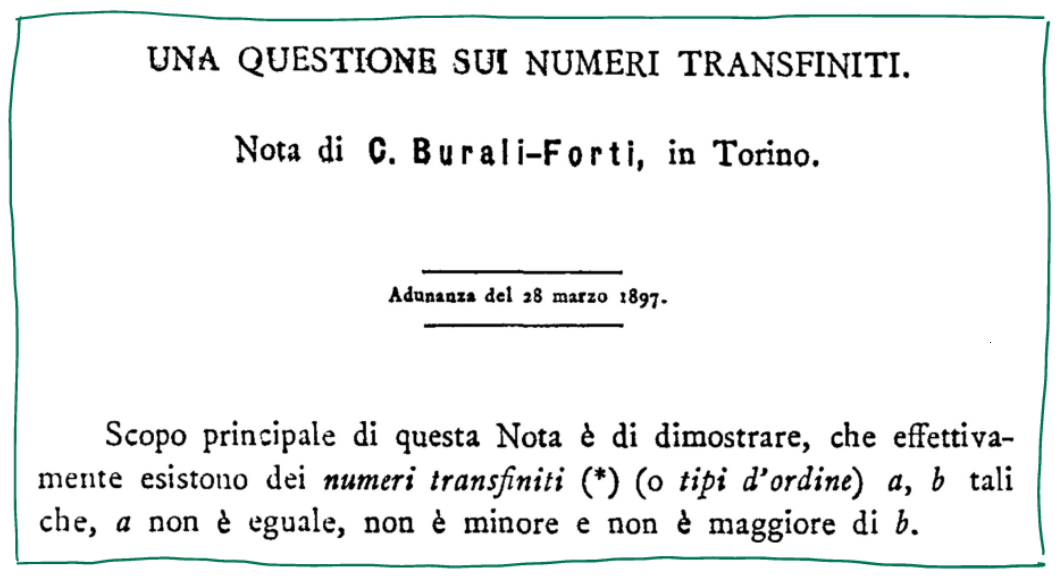
\includegraphics[width = 7.5cm]{immagini/Burali_Forti.png}
	\end{figure}
	Burali-Forti credette di poter negare la totalità dell'ordine $\prec$ ragionando per assurdo. Se $\prec$ fosse un ordine totale, si può dimostrare che è buono esattamente come abbiamo visto sopra, ma 
	allora $\Omega \Mydef [(\Ord,\prec)]$, la classe di isomorfismo di $(\Ord,\prec)$\footnote{Per la precisione stiamo prendendo l'ordinale associato, cosa che non sappiamo ancora fare ma che si può fare come vedremo a breve.},
	sarebbe a sua volta una classe di isomorfismo di un buon ordinamento e quindi uno dei membri della classe $\Ord$ stessa,
	e, considerando il suo successore $s(\Omega)$, avremmo $\Omega \prec s(\Omega)$, ma anche ovviamente $s(\Omega) \prec \Omega$, perché $s(\Omega) \in \Ord\;\textcolor{red}\lightning$.\\
	Il guaio è che, nello stesso anno, Cantor pubblicò una dimostrazione del fatto che la relazione $\prec$ è totale - esattamente l'argomento dei segmenti iniziali isomorfi che abbiamo illustrato 
	nel corso. Come è stata risolta la contraddizione? Concludendo che l'insieme di tutti gli ordinali esiste? \textcolor{red}{No}. Sfortunatamente Burali-Forti 
	aveva capito male la definizione di buon ordinamento, e ancora così, forse, nessuno se ne sarebbe accorto, ma, quel che è peggio, aveva tentato di correggerla, facendo, in realtà un pasticcio.
	La contraddizione è stata quindi imputata, da Burali-Forti e da Cantor, al bisticcio di definizioni ed il paradosso è stato dimenticato. Cinque anni dopo, \href{https://en.wikipedia.org/wiki/Bertrand_Russell}{\textcolor{purple}{Russell}}
	si rese conto del fatto che l'assurdo sussiste anche se si usa la definizione corretta di buon ordinamento, e fu così che il paradosso di Burali-Forti acquisì il suo nome. E tutti vissero felici e contenti.
\end{note}

\subsection{L'assioma del rimpiazzamento}
Gli ordinali di Von Neumann sono eleganti, ma quanti ne abbiamo di questi arnesi? Si può dimostrare che, assumendo i soli assiomi 1-7, il gran totale degli ordinali potrebbe essere:
\[ \textcolor{purple}{\Ord \overset{?}{=} \underbrace{\{\emptyset, s(\emptyset),\ldots,s^n(\emptyset),\ldots,\omega,s(\omega),\ldots,s^n(\omega),\ldots\}}_{\textnormal{\textcolor{MidnightBlue}{in realtà, questo si chiamerà $\omega + \omega$}}}}
	\]
la classe degli ordinali raggiungibili a partire da $\emptyset$ o da $\omega$ con un numero finito di applicazioni della mappa successore.

\begin{exercise}
	Dimostra che la classe descritta sopra è effettivamente una classe, ossia è definita da una formula.
\end{exercise}

\begin{soln}
	Chiamiamo $O = \{\emptyset, s(\emptyset),\ldots,s^n(\emptyset),\ldots,\omega,s(\omega),\ldots,s^n(\omega),\ldots\}$, allora la formula insiemistica che descrive $O$ è:
	\[ x \in O \Mydef (x = \emptyset) \lor (x = \omega) \lor (\exists n \in \omega \; (\underbrace{x = s^n(\emptyset)}_{x = n} \lor \underbrace{x = s^n(\omega)}_{x = \omega + n}))
		\]
	avendo una formula insiemistica ben posta, abbiamo che $O$ è una classe.
\end{soln}

Se vogliamo poter rispondere alla domanda ``quanti ordinali esistono?'' occorre un nuovo assioma: l'assioma del rimpiazzamento. Sotto questa ipotesi addizionale, la risposta sarà
``tutti quelli che potrebbero esistere'', ossia avremo un ordinale per ogni classe di isomorfismo di buoni ordini. Per formulare l'assioma, ci avvarremo dell concetto di funzione classe.

\begin{definition}[Funzione classe]
	Date due classi $A$ e $B$ una \vocab{funzione classe} da $A$ a $B$ è una formula insiemistica $\varphi(x,y)$ tale che:
	\[ \forall x \in A \;\exists \textcolor{red}{!}\,y \in B \; \varphi(x,y)
		\]
\end{definition}

\textcolor{MidnightBlue}{Ossia, una funzione classe è una proprietà, espressa nel linguaggio della teoria degli insiemi, che ad ogni $x \in A$ associa un \textcolor{red}{unico} $y \in B$.}

\begin{notation}[Funzione classe]
	Possiamo denotare una funzione classe $\varphi(x,y)$ da $A$ a $B$ mediante la notazione più familiare:
	\[ F : A \rightarrow B
		\]
	In questo caso, la scrittura $y = F(x)$ è una semplice abbreviazione:
	\[ y = F(x) \Mydef y \in B \land \varphi(x,y)
		\]
\end{notation}

\begin{example}[Esempi di funzioni classe]
	Le seguenti sono funzioni classe $V \rightarrow V$:
	\[ F_1(x) = x \qquad F_2(x) = \{x\} \qquad F_3(x) = \ps(x) \qquad F_4(x) = s(x)
		\]
	La funzione classe $F_5(x) = \sup(x \cap \Ord)$, con $x \cap \Ord \Mydef \{\alpha \in x | \alpha \in \Ord\}$, è $V \rightarrow \Ord$.
\end{example}

\begin{axiom}[Assioma del rimpiazzamento]
	\label{ax8}
	Se $A$ è un \textcolor{LimeGreen}{insieme} e $F : V \rightarrow V$ è una funzione classe, allora $F[A] \Mydef \{F(x) | x \in A\}$ è un \textcolor{LimeGreen}{insieme}.\footnote{Come per la separazione, anche questo è uno \vocab{schema di assiomi}, uno per ogni possibile (formula insiemistica) funzione classe $F$.}
	\[ \forall A \; \exists B \; \forall y \; y \in B \leftrightarrow \exists x \in A \; y = F(x)
		\]
	cioè per ogni insieme esiste un insieme i cui elementi sono immagini di quelli di $A$ per mezzo della funzione classe $F$.
\end{axiom}

\begin{proposition}[Unicità del rimpiazzo]
	Data una funzione classe $F : V \rightarrow V$ vale che:
	\[ \forall A \; \exists\textcolor{red}{!} B \; \forall y \; y \in B \leftrightarrow \exists x \in A \; y = F[x]
		\]
\end{proposition}

\begin{proof}
	Estensionalità.
\end{proof}

\begin{remark}[Rimpiazzamento da insieme a classe]
	Dato un \textcolor{red}{insieme} $A$ e una funzione classe $G : \textcolor{red}{A} \rightarrow V$, esiste ed è unico l'\textcolor{red}{insieme} $G[A]$ tale che:
	\[ \forall y \; y \in G[A] \leftrightarrow \exists x \in A \; y = G(x)
		\]
	in altre parole, l'assioma del rimpiazzamento vale anche con una funzione classe che va da un insieme ad una classe.
\end{remark}

\begin{proof}
	Ci basta semplicemente applicare l'\hyperref[ax8]{assioma del rimpiazzamento} appena enunciato, applicato alla funzione classe $F : V \rightarrow V$ definita come:
	\[ y = F(x) \Mydef (x \in A \land y = G(x)) \lor (x \not \in A \land y = \emptyset)
		\]
	ossia:
	\[ F(x) \Mydef \begin{cases}
		G(x) &\text{se $x \in A$} \\
		\emptyset &\text{altrimenti}
	\end{cases}
		\]
	infatti se $x \in A$ si ha $G(x) = F(x)$, altrimenti c'è il vuoto, per cui $G[A] = F[A]$ è un insieme grazie al rimpiazzamento.
\end{proof}

\begin{exercise}[Esistenza del prodotto cartesiano via rimpiazzamento]
	Dimostra che, dati due insiemi $A$ e $B$, esiste il loro prodotto cartesiano $A \times B$, usando l'assioma del rimpiazzamento ma \textcolor{red}{senza usare l'assioma delle parti}.
\end{exercise}

\begin{soln}
	L'idea è quella di creare l'insieme di tutti gli insiemi del tipo $\{\{a\},\{a,b\}\}$, per tutti gli $a \in A$ e $b \in B$. Per fare questo, fissato $b \in B$ definiamo la funzione classe:
	\[ H : V \to V : x \mapsto \{x,b\}
		\]
	che è ben definita per l'assioma del paio. Ora per rimpiazzamento $H[A] = A_b$ è un insieme \textcolor{MidnightBlue}{- ed è in particolare l'insieme di tutte le coppie $\{a,b\}$ al variare di $a \in A$ -},
	ora possiamo definire la funzione classe:
	\[ G : A_b \to V : \{a,b\} \mapsto \{\{a\},\{a,b\}\}
		\]
	che è ben definita perché di fatto stiamo facendo $\{\{a,b\}\cap A\} \cup \{\{a,b\}\}$, che è ancora un insieme per gli assiomi di singoletto e unione. A questo punto $E_b = G[A_b]$ 
	è un insieme per rimpiazzamento \textcolor{MidnightBlue}{- ed è proprio l'insieme di tutti gli insiemi $\{\{a\},\{a,b\}\}$ per $b$ fissato e $a$ che varia in $A$, cioè è proprio $A \times \{b\}$ -}.
	A questo punto possiamo definire la funzione classe:
	\[ F : B \to V : b \mapsto E_b
		\]
	che è ben definita per quanto osservato e $F[B] = C$ che ci dà l'insieme $\{E_b\}_{b \in B} = \{\{A \times \{b\}\}\}_{b \in B}$ , da cui:
	\[ \bigcup C
		\]
	è l'insieme, per l'assioma dell'unione, di tutte le coppie ordinate $(a,b)$ per $a \in A$ e $b \in B$, ed è quindi proprio $A \times B$.
\end{soln}

\begin{theorem}[Ogni buon ordine è isomorfo ad un unico ordianle]
	Dato un buon ordine $(A,<)$, esiste un unico ordinale $\alpha$ tale che $(A,<)\sim\alpha$.
\end{theorem}

\begin{proof}
	L'unicità segue per quanto abbiamo già visto, cioè $\alpha \sim \alpha' \rightarrow \alpha = \alpha'$. Basta quindi da dimostrare l'esistenza di almeno un ordinale $\alpha$ per ogni classe di isomorfismo di un buon ordinamento. Sia:
	\[ A' = \{x \in A | \exists \gamma \in \Ord \; A_x \sim \gamma\}
		\]
	ovvero l'insieme degli elementi nel buon ordinamento che determinano segmenti iniziali isomorfi ad un qualche ordinale.
	Consideriamo la funzione classe $F : A' \rightarrow \Ord$:
	\[ F(x) = \text{l'unico $\gamma \in \Ord$ tale che $A_x \sim \gamma$}
		\]
	l'unicità segue dalla solita proposizione e ci garantisce che la funzione classe sia ben definita:
	\[ A_x \sim \gamma \land A_x \sim \gamma' \implies \gamma \sim \gamma' \implies \gamma = \gamma'
		\]
	Vogliamo dimostrare che l'insieme $\alpha := F[A'] \sim (A,<)$ - che esiste per rimpiazzamento - è proprio un ordinale isomorfo a $(A,<)$.
	Dimostriamo dunque che $\alpha$ è un ordinale, $A'$ è un segmento iniziale di $A$, $\alpha \sim A'$, e infine che $A' = A$.
	\begin{itemize}
		\item[$\boxed{\text{$\alpha$ è un ordinale}}$] $\alpha$ è definito come l'insieme degli ordinali isomorfi ai segmenti iniziali corrispondenti agli elementi di $A'$, dunque, per un fatto visto, ci basta dimostrare che è transitivo affinché sia un ordinale a sua volta.\\
		Sia $\gamma \in \beta \in \alpha$, con $\beta$ che è per definizione un ordinale isomorfo ad un qualche segmento iniziale principale di $A$, $\beta \sim A_a$, vediamo che anche $\gamma$ è isomorfo ad un segmento iniziale principale di $A$ e quindi $\gamma \in \alpha$.
		Fissato un isomorfismo $f : \beta \to A_a$, possiamo considerarne la restrizione a $\gamma$, che è ancora un isomorfismo, $f_{|\gamma} : \gamma \to (A_a)_{f(\gamma)} = A_{f(\gamma)}$, dove abbiamo usato che gli isomorfismi mandano s.i. in s.i., $f[\gamma] = f[\beta_\gamma] = (A_a)_{f(\gamma)}$, abbiamo quindi ottenuto che $\gamma = F(f(\gamma))$.
		\item[$\boxed{\text{$A'$ s.i. di $A$}}$] Sia $y < x \in A'$, vogliamo verificare che $y \in A'$, poiché $x \in A'$ esiste $\gamma \in \Ord$ tale che $A_x \sim \gamma$, e naturalmente $A_y \subsetneq A_x$. Fissato $f : A_x \to \gamma$ isomorfismo, se verifichiamo che $f[A_y]$ è un ordinale abbiamo concluso poiché si avrebbe $A_y \sim f[A_y] \in \Ord$ e quindi $y \in A'$.
		A questo punto dati $\beta \in \alpha \in f[A_y]$, poiché $A_y$ è un isomorfismo, tornando indietro si ha $f^{-1}(\beta) < f^{-1}(\alpha) \in A_y$, ma poiché $A_y$ è un segmento iniziale, allora $f^{-1}(\beta) \in A_y \iff \beta \in f[A_y]$.\\
		\textcolor{MidnightBlue}{\underline{Alternativa}: Fissato $f : A_x \to \gamma$ isomorfismo, allora $f_{|A_y} : A_y \to \gamma_{f(y)}$ è un isomorfismo perché restrizione di un isomorfismo e sappiamo che gli isomorfismi mandano segmenti iniziali principali in segmenti iniziali principali per un'osservazione vista in precedenza, dunque l'immagine è proprio $\gamma_{f(y)}$, inoltre
		$\gamma_{f(y)} = f(y) \in \Ord$, quindi evitiamo la verifica diretta che l'immagine sia un ordinale.}
		\item[$\boxed{A' \sim \alpha}$] Sia $f : A' \rightarrow \alpha = F[A'] : x \mapsto F(x)$ la funzione tra insiemi, definita per separazione in $A' \times \alpha = A' \times F[A']$ - quindi abbiamo prima ottenuto l'insieme di arrivo con rimpiazzamento e poi ci siamo ristretti a quest'ultimo per avere una funzione -. Dimostriamo che $f$ è un isomorfismo di ordini.\\
		La surgettività è immediata perché, per costruzione, abbiamo che $\alpha = F[A'] \overset{\text{def. $f$}}{=} f[A']$. Osserviamo ora che la stretta crescenza deriva dall'ordinamento dei segmenti iniziali:
		\[ x <_A y \implies f(x) \sim A_x \prec A_y \sim f(y)
			\]
		dove gli isomorfismi sono per definizione di $f$, e la disuguaglianza tra i segmenti iniziali come buoni ordinamenti deriva banalmente da $x < y$. Segue quindi che $f(x) \prec f(y)$, ed essendo ordinali ciò significa proprio che $f(x) \in f(y) \equiv f(x) < f(y)$.
		\item[$\boxed{A' = A}$] Se $A' \ne A$, cioè se $A' \subsetneq A$, avendo visto che $A'$ è un segmento iniziale, abbiamo che è principale, quindi $A' = A_k$, per $k \in A$.		Ma allora $A_k \sim \alpha \in \Ord$ per i punti 1. e 3., per cui $k \in A' = A_k \;\textcolor{red}\lightning$.
	\end{itemize}
\end{proof}

Una conseguenza del risultato precedente è che possiamo definire le operazioni sugli ordinali come semplice riflesso di quelle sui buoni ordini - avendo a questo punto una corrispondenza esatta tra classi di isomorfismo di buoni ordini e ordinali -.

\begin{definition}[Operazioni sugli ordinali - v.1]
	Dati $\alpha,\beta \in\Ord$, definiamo \vocab{$\alpha + \beta$}, \vocab{$\alpha\cdot\beta$}, \vocab{$\alpha^\beta$} come, rispettivamente, l'unico ordinale tale che:
	\[ \textcolor{purple}{\alpha + \beta} \sim (\alpha,<_\alpha)+(\beta,<_\beta) \qquad \textcolor{purple}{\alpha \cdot \beta} \sim (\alpha,<_\alpha) \cdot (\beta,<_\beta)
		\]\[ \textcolor{purple}{\alpha^\beta} \sim (\alpha,<_\alpha)^{(\beta,<_\beta)}
			\]
\end{definition}

\begin{exercise}
	Dimostra che l'insieme introdotto all'inizio della sezione è effettivamente $\omega + \omega$, ossia, più precisamente:
	\[ \forall x \; x \in \omega + \omega \leftrightarrow (\exists m \in \omega \; x = m) \lor (\exists n \in \omega \; x = \omega +n)
		\]
\end{exercise}

\begin{soln}
		
\end{soln}


\pagebreak
\subsection{Induzione e ricorsione transfinite}
Il piatto forte di questa sezione è una seconda applicazione dell'assioma del rimpiazzamento: il teorema di ricorsione transfinita. Questo risultato sarà più chiaro a chi ha, in precedenza, risolto il seguente esercizio.

\begin{exercise}
	Dimostra che esiste un insieme $A$ tale che:
	\[ \forall x \; x \in A \leftrightarrow x = \emptyset \lor \exists y \in A \; x = \{y\}
		\]
	\textcolor{MidnightBlue}{ossia, in sostanza dimostra che esiste:}
	\[ \textcolor{MidnightBlue}{\{\emptyset,\{\emptyset\},\{\{\emptyset\}\},\{\{\{\emptyset\}\}\},\ldots\}}
		\]
	\textcolor{MidnightBlue}{ovvero un insieme che contiene $\emptyset$ e tale per cui qualsiasi altro elemento diverso dal vuoto che contiene è il singoletto di un altro suo elemento.}
\end{exercise}

L'idea per risolvere questo esercizio è contenuta nella dimostrazione del teorema di ricorsione \textcolor{red}{numerabile}, che abbiamo già visto. Attenzione, però,
che questo teorema non si può applicare dire alla situazione dell'esercizio - perché non abbiamo un insieme in arrivo -.

\begin{soln}
	Vorremmo definire la funzione classe $F : \omega \to V$ data da:
	\[ \text{$F(n) =$ singoletto $n$ volte di $\emptyset$}
		\]
	a questo punto potremmo verificare che $A = F[\omega]$ soddisfa la richiesta. Occorre quindi dimostrare che la definizione informale di $F$ data sopra è esprimibile nel linguaggio formale della teoria degli insiemi.
	Diamo la seguente definizione per $n \in \omega$ abbiamo:
	\[ y = F(n) := \exists f \;\text{tale che } \begin{cases}
		\text{$f$ è una funzione} \\
		\Dom(f) = s(n) \\
		f(0) = \emptyset \\
		\forall i \in n \; f(s(i)) = \{f(i)\} \\
		f(n) = y
	\end{cases}
		\]	
	\textcolor{MidnightBlue}{(notare che le tre richieste nel mezzo sono identiche alla definizione di $n$-approssimazione, nonché $f(n) = y$ è proprio il modo in cui dalle approssimazioni passiamo alla ricorsione nel teorema di ricorsione numerabile)}
	cioè fissato $n \in \omega$, dire $y = F(n)$, vuol dire che esiste una funzione $f$ con le proprietà richieste sopra, che calcolata in $n$ dà appunto $y$ (cioè il vuoto con $n$ parentesi).\\
	Proprio come nel teorema di ricorsione numerabile, per dimostrare che $F$ è una funzione classe, ci basta dimostrare che $\forall n \in \omega \; \exists\textcolor{red}!f$ che soddisfa le tre richieste centrali, fatto ciò
	$f$ sarà ben definita ed unica - per cui sarà ben definito anche $f(n) = y$ -, e quindi anche $F$ è ben posta \textcolor{MidnightBlue}{- in pratica esistono e sono uniche le approssimazioni finite anche in questo caso, e come nel teorema di ricorsione numerabile possiamo costruire una funzione (classe in questo caso) che unisce le approssimazioni finite}.
	\begin{itemize}
		\item[$\boxed{\text{esistenza}}$] Procediamo per induzione numerabile. Il caso $n = 0$ è immediato, basta considerare $f = \{(0,\emptyset)\}$ e tale $f$ rispetta tutte le richieste.\\
		Nel caso $n = s(m)$, per ipotesi induttiva, abbiamo una funzione $f'$ con $\Dom(f') = n$, $f'(0) = \emptyset$ e $\forall i < n \; f'(s(i)) = \{f'(i)\}$.
		Poniamo quindi $f = f' \cup \{(n,\{f'(m)\})\}$ ed otteniamo che $\Dom(f) = \Dom(f') \cup \{n\} = s(n)$, $f(0) = f'(0) = \emptyset$ e, preso $i < n = s(m)$, o $i < m$ o $i = n$;
		nel primo caso abbiamo che $f(s(i)) = f'(s(i)) = \{f'(i)\} = \{f(i)\}$, nel secondo $f(s(i)) = f(n) = \{f'(m)\} = \{f(m)\} = \{f(i)\}$.
		\item[$\boxed{\text{unicità}}$] Date $f_1$ e $f_2$ che soddisfano le condizioni: $\Dom(f_*) = s(n)$, $f_*(0) = \emptyset$ e $\forall i < n \; f_*(s(i)) = \{f_*(i)\}$, dimostriamo per induzione su $i$ che $\forall i \in \omega \; i \leq n \to f_1(i) = f_2(i)$.
		\begin{itemize}
			\item \underline{Caso $i = 0$}: $f_1(0) = \emptyset = f_2(0)$.
			\item \underline{Caso $i = s(j)$}: $f_1(i) = \{f_1(j)\} \overset{\text{Hp. indutt.}}{=} \{f_2(j)\} = f_2(i)$.
		\end{itemize}
	\end{itemize}
	Ora che abbiamo la funzione classe $F$ - abbiamo verificato che l'immagine della formula insiemistica data esiste ed è unica - è immediato verificare che $F(0) = \emptyset$. Inoltre, dato $n \in \omega$, $F(s(n)) = \{F(n)\}$, infatti, detto $y = F(s(n))$,
	per definizione esiste ed è unica $f$ la funzione con $\Dom(f) = s(s(n)),\ldots$ tale che $F(s(n)) = f(s(n))$, osserviamo che $f_{|s(n)}(n) = F(n)$ (si verifica facilmente che $f_{|s(n)}$ rispetta tutte le richieste della definizione di $y = F(n)$, e quindi è proprio l'unica funzione che esiste per tale definizione). Abbiamo quindi:
	\[ F(s(n)) = f(s(n)) \overset{\text{def. $f$}}{=} \{f(n)\} = \{F(n)\}
		\]
	Abbiamo quindi che $F$ - oltre ad essere ben definita ed unica - soddisfa anche le richieste che volevamo per poter dire ``singoletto di $\emptyset$ $n$ volte'', a questo punto possiamo quindi considerare
	$A:=F[\omega]$ ed osservare che è proprio l'insieme che stavamo cercando. Infatti $\emptyset = F(0) \in A$, e, preso $y \in A = F[\omega]$ che non sia il vuoto, abbiamo $y = F(n)$, con $n \ne 0$, per cui $n = s(m)$,
	per qualche $m \in \omega$, allora detto $x = F(m) \in A$, si ha $y = F(s(m)) \overset{\text{oss. prima}}{=} \{F(m)\} = \{x\}$, pertanto qualsiasi elemento non sia il vuoto 
	è il singoletto di qualche altro elemento dell'insieme, proprio come richiesto dalla formula nella richiesta.
\end{soln}

\begin{proposition}[Induzione transfinita - v.1]
	\label{induz_transf1}
	Data una formula insiemistica $\varphi(x)$. Se vale [l'ipotesi dell'induzione]\footnote{Come nell'induzione normale, il difficile sta nel mostrare che vale il passo induttivo, rappresentato dall'implicazione nell'ipotesi, poi il teorema assicura la veridicità dell'enunciato.}:
	\[ \forall \alpha \in \Ord(\forall \beta < \alpha \; \varphi(\beta))\rightarrow \varphi(\alpha)
		\]
	ovvero se per ogni ordinale, sapere che la formula è vera per gli ordinali più piccoli, rende vera la formula per l'ordinale stesso, allora la formula vale per tutti gli ordinali $\forall \alpha \in \Ord \; \varphi(\alpha)$.
\end{proposition}

\textcolor{MidnightBlue}{In termini di classi, rappresentando con $C$ la classe definita dalla formula $\varphi(x)$, abbiamo che se vale $\forall\alpha\in\Ord \;(\forall \beta < \alpha \; \varphi(\beta))\rightarrow \alpha \in C$,
allora $\forall \alpha \in \Ord \; \alpha \in C$, cioè $\Ord \subseteq C$.}

\begin{proof}
	Per assurdo, neghiamo la tesi $\neg(\forall \alpha \in\Ord\;\varphi(\alpha)) \equiv \exists \alpha \in \Ord \;\neg\varphi(\alpha)$. Possiamo quindi fissare un $\alpha$ per cui la formula $\varphi(\alpha)$ è falsa,
	a questo punto, applicando l'ipotesi ad $\alpha$, dovendo essere l'implicazione sempre vera, ed avendo conseguente falso - ovvero $\varphi(\alpha)$ -, allora anche l'antecedente deve essere falso, ovvero deve necessariamente valere che $\neg(\forall \beta < \alpha \; \varphi(\beta)) \equiv \exists \beta < \alpha \; \neg \varphi(\beta)$.\\
	Reiterando lo stesso identico ragionamento con $\beta$, otteniamo che esiste almeno un $\gamma < \beta$ tale che è vera $\neg \varphi(\gamma)$, per cui possiamo considerare $\beta_0 := \min\{\gamma \in \beta | \neg \varphi(\gamma)\}$\footnote{Ora possiamo scrivere un insieme per separazione in $\beta$ - prima non potevamo essendo $\alpha \in \Ord$ - non vuoto per quanto visto, e quindi con un minimo per le proprietà degli insiemi di ordinali.}
	Reiterando di nuovo il ragionamento iniziale con $\beta_0$ otteniamo che esiste almeno un $\delta < \beta_0$ tale che è vera $\neg\varphi(\delta)$, contro la minimalità di $\beta_0 \; \textcolor{red}\lightning$.
\end{proof}

\begin{note}[L'induzione transfinita è uno schema di teoremi]
	Il principio di induzione transfinita non è, letteralmente, un teorema della teoria degli insiemi, quanto piuttosto uno scherma di teoremi - o metateorema - che ci permette 
	di costruire un diverso teorema per ogni possibile formula $\varphi$ nel linguaggio della teoria degli insiemi - non essendo le classi oggetti della teoria degli insiemi, esse non possono essere quantificate con i quantificatori soliti, quindi l'induzione può
	essere enunciata solo per una formula fissata ogni volta, e non per tutte le formule -.
\end{note}

C'è una chiara analogia fra la forma precedente del principio di induzione transfinita e la forma forte dell'induzione aritmetica.
A volte, però, è comodo esprimere l'induzione transfinita in una forma che meglio ricorda il principio di induzione di Peano.

\begin{definition}[Ordinali successori e limiti]
	Diciamo che $\alpha \in \Ord$ è un \vocab{ordinale successore} se $\exists \beta \in \Ord \; \alpha = s(\beta)$. Un ordinale $\alpha\;\textcolor{red}{> 0}$ che non è successore è detto \vocab{ordinale limite}.
\end{definition}

\begin{remark}[Caratterizzazione degli ordinali successori]
	Un ordinale $\alpha$ è successore se e solo se ha un massimo.\footnote{Più precisamente, un insieme di ordinali è un ordinale successore se e solo se è transitivo ed ha un massimo. Equivalentemente un ordinale che non ha massimo è limite.}
\end{remark}

\begin{proof}
	Ci basta osservare che vale la seguente catena di equivalenze:
	\[ \text{$\beta$ è il massimo di $\alpha$} \iff \text{$\alpha$ è il minimo ordinale $> \beta$} \iff s(\beta) = \alpha
		\]
	la seconda equivalenza l'abbiamo già vista in precedenza, dimostriamo quindi la prima.
	\begin{itemize}
		\item[$\boxed{\Longleftarrow}$] Se $\beta$ non fosse il massimo di $\alpha$, allora esisterebbe un ordinale $\gamma$ tale che $\alpha > \gamma > \beta$, che è contro la minimalità di $\alpha$.
		\item[$\boxed{\Longrightarrow}$] Se esistesse un ordinale $\gamma$ più grande di $\beta$ e più piccolo di $\alpha$, $\beta < \gamma < \alpha$, si avrebbe che $\gamma \in \alpha$ supera $\beta$ che quindi non può essere il massimo di $\alpha$.
	\end{itemize}
\end{proof}

\begin{proposition}[Induzione transfinita - v.2]
	\label{induz_transf2}
	Sia $\varphi(x)$ una formula insiemistica, se vale:
	\begin{enumerate}[(i)]
		\item $\varphi(0)$ \textcolor{orange}{(caso base)}
		\item $\forall \gamma \in \Ord \; \varphi(\gamma) \rightarrow \varphi(s(\gamma))$ \textcolor{orange}{(caso successore)}
		\item per ogni ordinale limite $\lambda$ si ha $(\forall \beta < \lambda \; \varphi(\beta)) \rightarrow \varphi(\lambda)$\footnote{Cioè vale anche un passo induttivo - forte - per gli ordinali che non sono successori.} \textcolor{orange}{(caso limite)}
	\end{enumerate}
	allora $\forall \alpha \in \Ord \; \varphi(\alpha)$.
\end{proposition}

\begin{proof}
	Basta verificare l'ipotesi della prima forma dell'\hyperref[induz_transf1]{induzione transfinita}, per avere in automatico la veridicità della formula in generale. Fissato quindi $\alpha \in \Ord$ bisogna mostrare che vale la formula:
	\[ (\forall \beta < \alpha \; \varphi(\beta)) \rightarrow \varphi(\alpha)
		\]
	Se $\alpha$ è limite o $0$ abbiamo questa formula tout court - nel caso di 0 la formula sopra è vera a vuoto, nel caso degli ordinali limite abbiamo assunto che la formula sopra è vera come ipotesi -. Verifichiamo che la formula sopra è vera anche
	nel caso in cui $\alpha = s(\gamma)$:
	\[ \forall \beta < \alpha \;\textcolor{LimeGreen}{= s(\gamma)} \; \varphi(\beta) \overset{\textcolor{purple}{\gamma < s(\gamma)}}{\implies} \varphi(\gamma) \overset{\text{Hp. (ii)}}{\rightarrow} \varphi(s(\gamma)) = \varphi(\alpha)
		\]
	dunque anche in questo caso vale l'ipotesi della prima forma dell'induzione transfinita, che quindi vale proprio $\forall \alpha \in \Ord$. Pertanto la prima forma dell'induzione transfinita ci garantisce che $\varphi(\alpha)$ vale per tutti gli $\alpha \in \Ord$.
\end{proof}

Ora possiamo finalmente dimostrare il teorema di ricorsione transfinita.

\begin{notation}[Restrizione di una funzione classe a funzione]
	Data una funzione classe $F : A \rightarrow B$ e un insieme $X \subseteq A$ esiste la funzione tra insiemi:
	\[ f = F_{|X} : X \rightarrow F[X] : a \mapsto F[a]
		\]
	che è ottenuta per separazione in $X \times F[X]$ - il secondo è un insieme per rimpiazzamento -, ed è in automatico una funzione surgettiva.
\end{notation}


\begin{theorem}[Ricorsione transfinita - v.1]
	\label{ric_transf1}
	Data una funzione classe $G : V \rightarrow V$ esiste un'unica\footnote{Dove l'unicità va intesa nel senso seguente: date $F_1,F_2$ come sopra, vale $\forall \alpha \in \Ord \; F_1(\alpha) = F_2 (\alpha)$.} funzione $F : \Ord \rightarrow V$ tale che:
	\[ \forall \alpha \in \Ord \; F(\alpha) = G(F_{|\alpha})
		\]
\end{theorem}

\textcolor{MidnightBlue}{L'idea è di costruire una funzione classe $H : \Ord \to V$ - la successione delle troncate di $G$ - in maniera tale che, a posteriori, avremo $F_{|\alpha} = H(\alpha)$. Poi semplicemente porremo $F(\alpha) := H(s(\alpha))(\alpha)$.
$H(\alpha)$ è l'analogo transfinito di una $\alpha$-approssimazione nella dimostrazione del teorema di ricorsione numerabile -nel senso della seconda forma più che della prima\footnote{Anzi, di fatto, questa dimostrazione rimaneggiata ci dà una dimostrazione del secondo teorema di ricorsione numerabile usando le approssimazioni finite.} -.}

\begin{proof}
	Definiamo la funzione classe $H : \Ord \to V$ con:
	\[ f = H(\alpha) := \begin{cases}
		\text{$f$ è una funzione} \\
		\Dom(f) = \alpha \\
		\forall \beta \in \alpha \; f(\beta) = G(f_{|\beta})
	\end{cases}
		\]
	Verifichiamo, per induzione  transfinita su $\alpha$, che $H$ sia realmente una funzione classe $\Ord \to V$, ossia che sia effettivamente una funzione:
	\[ \forall \alpha \in \Ord \; \exists\textcolor{red}{!}f \; f = H(\alpha)
		\]
	\begin{itemize}
		\item[$\boxed{\text{caso 0}}$] $f = H(0) \iff f = \emptyset$, quindi $f$ esiste ed è unica quando si valuta $H$ in 0.
		\item[$\boxed{\text{caso $\alpha = s(\gamma)$}}$] Per ipotesi induttiva esiste ed è unica $f = H(\gamma)$, dunque possiamo definire $f' = f \cup \{(\gamma,G(f))\}$ e verificare che $f'$ rispetta le condizioni ed è unica.
		Si vede immediatamente che $\Dom(f') = \Dom(f) \cup \{\gamma\} = \gamma \cup \{\gamma\} = s(\gamma) = \alpha$, inoltre, preso $\beta \in \alpha = s(\gamma)$ si hanno due casi:
		\begin{itemize}
			\item[$\diamondsuit$] \underline{se $\beta \in \gamma$}: allora $f'(\beta) \overset{\text{def.}}{=} f(\beta) \overset{\text{Hp. indutt.}}{=} G(f_{|\beta}) \overset{\text{def.}}{=} G(f'_{|\beta})$
			\item[$\diamondsuit$] \underline{se $\beta = \gamma$}: allora $f'(\gamma) \overset{\text{def.}}{=} G(f) = G(f_{|\gamma}) \overset{\text{def.}}{=} G(f'_{|\gamma})$, dove l'uguaglianza al centro vale poiché banalmente $f = f_{|\gamma}$ essendo $\Dom(f) = \gamma$.
		\end{itemize}
		Verifichiamo ora l'unicità di $f'$, data $g = H(\alpha)$ - cioè un'altra funzione che rispetta le condizioni iniziali -, siccome $\Dom(f') = \Dom(g) = \alpha$, ci basta verificare che le due funzioni coincidono su $\alpha$.
		Per definizione $g_{|\gamma} = H(\gamma)$ e per l'unicità di $f$ si ha che $g_{|\gamma} = f = f'_{|\gamma}$, l'unico caso che resta da verificare è quindi $\gamma$ stesso:
		\[  g(\gamma) \overset{\text{def.}}{=} G(g_{|\gamma}) \overset{\text{Hp. indutt.}}{=} G(f) = G(f'_{|\gamma}) \overset{\text{def.}}{=} f'(\gamma)
			\]
		\item[$\boxed{\text{caso $\alpha = \lambda$}}$] Sia $\lambda$ limite, per ipotesi induttiva abbiamo che $\forall \beta < \lambda \;\exists\textcolor{red}{!}f \; f = H(\beta)$ tale che $\Dom(f) = \beta$ e $\forall \gamma < \beta \; f(\gamma) = G(f_{|\gamma})$, dobbiamo dimostrare che $\exists\textcolor{red}{!}g \; g = H(\lambda)$, con $\Dom(g) = \lambda$ e $\forall \beta < \lambda \; g(\beta) = G(g_{|\beta})$.\\
		Per rimpiazzamento esiste l'insieme $H[\lambda]$, poniamo $h := \bigcup H[\lambda] = \bigcup_{\beta < \lambda} H(\beta)$, vogliamo dimostrare che $g = H(\lambda) \leftrightarrow g = h$. Per cominciare dimostriamo che $h = H(\lambda)$.
		\begin{itemize}
			\item[$\diamondsuit$] \underline{$h$ è una funzione}: Dobbiamo dire che date $f_1,f_2 \in H[\lambda]$, queste coincidono sull'intersezione dei loro domini. Siano $f_1 = H(\beta_1)$ e $f_2 = H(\beta_2)$,
			assumiamo WLOG che $\beta_1 < \beta_2$, segue quindi che $f_{2|\beta_1} = H(\beta_1)$ - per definizione la restrizione di $f_2$ rispetta le proprietà di una $\beta_2$-approssimazione, e per ipotesi induttiva è unica (ed è proprio $H(\beta_2)$), quindi $f_{2|\beta_1} = H(\beta_1) = f_2 $.
			\item[$\diamondsuit$] \underline{$\Dom(h) = \lambda$}: Segue banalmente che:
			\[ \Dom(h) = \bigcup_{\beta \in \lambda} \Dom(H(\beta)) = \bigcup_{\beta \in \lambda} \beta = \lambda
				\]
			\item[$\diamondsuit$] \underline{$\forall \beta < \lambda \; h(\beta) = G(h_{|\beta})$}: Dato $\beta < \lambda$, essendo $\lambda$ limite, $s(\beta) < \lambda$, quindi, detta $f = H(s(\beta))$ \textcolor{MidnightBlue}{- di fatto è la più piccola funzione che calcola $f(\beta)$ e le altre che lo calcolano nell'unione 
			sono sue estensioni -}, abbiamo $h(\beta) \overset{\text{def. $h$}}{=} f(\beta) \overset{\text{Hp. indutt.}}{=} G(f_{|\beta}) \overset{\text{def. $h$}}{=} G(h_{|\beta})$.
		\end{itemize}
		Abbiamo quindi che $h$ è una $\lambda$-approssimazione, verifichiamo l'unicità. Detta $g = H(\lambda)$, dobbiamo dimostrare che $\textcolor{purple}{g = h}$.
		Dato $\beta < \lambda$, abbiamo per definizione $g_{|\beta} = h_{|\beta} = H(\beta)$, e per l'unicità di $H(\beta)$ - che abbiamo per ipotesi induttiva - segue:
		\[ \forall \beta < \lambda \; g(\beta) = G(g_{|\beta}) = G(H(\beta)) = G(h_{|\beta}) = h(\beta) \implies g = h
			\]
	\end{itemize}
	Abbiamo stabilito che $H$ è una funzione classe ben posta. Definiamo ora:
	\[ y = F(\alpha) := \exists f \; f = H(s(\alpha)) \land y = f(\alpha)
		\]
	e per quanto abbiamo appena visto $F$ è ben definita poiché $H(s(\alpha))$ esiste ed è unica per ogni $\alpha \in \Ord$ \textcolor{MidnightBlue}{- in pratica $H$ è la successione delle troncate come nel secondo teorema di ricorsione numerabile -},
	dobbiamo quindi mostrare che $F(\alpha) = G(F_{|\alpha})$, infatti come nella ricorsione numerabile v.2, $F(\alpha) = f(\alpha) = (H(s(\alpha)))(\alpha) = G(f_{|\alpha})$, dunque ci basta solo verificare che $F_{|\alpha} = f_{|\alpha}$ per concludere l'esistenza.\\
	Preso $\beta < \alpha$ e $f' = H(s(\beta))$, per definizione che $F(\beta) \overset{\text{def. $F$}}{=} f'(\beta) = G(f'_{|\beta}) \;\textcolor{red}{=}\; G(f_{|\beta}) = f(\beta)$ dove l'uguaglianza in rosso vale perché le funzioni date da $H(\cdot)$ coincidono sull'intersezione dei loro domini per l'unicità delle approssimazioni vista sopra - fondamentalmente ciò ci 
	dice che le approssimazioni estendono ciascuna le altre\footnote{Per la precisione $f_{|\beta} = H(\alpha)_{|\beta} =$ unica $\beta$-approssimazione $= H(\beta) = H(s(\beta))_{|\beta} = f'_{|\beta}$ (poiché le restrizioni soddisfano ancora le proprietà delle approssimazioni).} -, pertanto $\forall \beta < \alpha \; F(\beta) = f(\beta) \implies F_{\alpha|} = f_{|\alpha}$. A questo punto si ha proprio $F(\alpha) = f(\alpha) = G(f_{|\alpha}) = G(F_{|\alpha})$.\\
	Resta da dimostrare l'unicità di $F$. Ossia che date $F_1$ e $F_2$ tali che:
	\begin{align*}
		&\forall \alpha \in \Ord \; F_1(\alpha) = G(F_{1|\alpha}) \\
		&\forall \alpha \in \Ord \; F_2(\alpha) = G(F_{2|\alpha})
	\end{align*}
	allora $\forall \alpha \in \Ord \; F_1(\alpha) = F_2(\alpha)$. Per \hyperref[induz_transf1]{induzione transfinita v.1} possiamo assumere che $\forall \beta < \alpha \; F_1(\beta) = F_2(\beta)$,
	ma questo equivale proprio a dire $F_{1|\alpha} = F_{2|\alpha}$, quindi:
	\[ F_1(\alpha) \overset{\text{def.}}{=} G(F_{1|\alpha}) \overset{\text{Hp. induttiva}}{=} G(F_{2|\alpha}) \overset{\text{def.}}{=} F_2(\alpha)
		\]
\end{proof}

Come per l'induzione, possiamo esprimere la ricorsione transfinita separando i casi zero, successore e limite.

\begin{definition}[Prodotto cartesiano  di classi]
	Date due classi $A,B$ definiamo la \vocab{classe prodotto cartesiano} $A \times B$ come:
	\[ x \in A \times B \Mydef \exists a \in A \; \exists b \in B \; x = (a,b)
		\]
\end{definition}

\begin{corollary}[Ricorsione transfinita - v.2]
	\label{ric_transf2}
	Date le funzioni classe $G_1 : \Ord \times V \rightarrow V$ e $G_2 : V \rightarrow V$ e dato $x_0 \in V$, esiste un'unica funzione classe $F : \Ord \to V$ tale che:
	\[ \forall \alpha \in \Ord \; F(\alpha) :=\begin{cases}
		F(0) = x_0 \\
		\forall \alpha \in \Ord \; F(s(\alpha)) = G_1(\alpha,F(\alpha)) \\
		\forall \lambda \in \Ord \; \text{$\lambda$ limite} \rightarrow F(\lambda) = G_2(F_{|\lambda})
	\end{cases}
		\]
\end{corollary}

\begin{proof}
	Ci basta applicare il \hyperref[ric_transf1]{teorema di ricorsione transfinita v.1}, e per farlo, non dobbiamo far altro che definire una funzione classe $G : \Ord \rightarrow \Ord$, rispetto a cui $F(\alpha) = G(F_{|\alpha})$, ed il teorema ci assicura esistenza ed unicità.
	Possiamo esibire $G$ nel modo seguente:\footnote{Il caso $f = \emptyset$ corrisponderebbe alla troncata 0-esima della ricorsione - come nella ricorsione numerabile $f'(0) = 0$, $f'(s(n)) = f'(n) \cup \{(n,h(f'(n)))\}$ e $f(0) = f'(s(0))(0) = h(0)$ -, per in maniera simile abbiamo $F(0) = G(F_{|0}) = G(\emptyset) = x_0$.}
	\[ G(f) = \begin{cases}
		\emptyset &\text{se $f$ NON è una funzione con $\Dom(f) \in \Ord$} \\
		x_0 &\text{se $f = \emptyset$ (o $\Dom(f) = \emptyset$)} \\
		G_1(\alpha,f(\alpha)) &\text{se $\Dom(f) = \alpha + 1$ per qualche $\alpha \in \Ord$} \\
		G_2(f) &\text{altrimenti}
	\end{cases}
		\]
\end{proof}

\subsection{Operazioni fra gli ordinali}

\begin{definition}[Operazioni sugli ordinali - v.2]
	Esistono le funzioni classe di somma, prodotto e potenza di ordinali, così definite:
	\[ \alpha + \beta :=\begin{cases}
		\alpha + 0 = \alpha \\
		\alpha + s(\beta) = s(\alpha + \beta) \\
		\alpha^\lambda = \sup\{\alpha + \beta | \beta < \lambda\} 
	\end{cases}
	\qquad
	\alpha \cdot \beta :=\begin{cases}
		\alpha \cdot 0 = 0 \\
		\alpha \cdot s(\beta) = \alpha \cdot \beta + \alpha \\
		\alpha\cdot \lambda = \sup\{\alpha \cdot \beta | \beta < \lambda\}
	\end{cases}
		\]
	\[ \alpha^\beta :=\begin{cases}
		\alpha^0 = 1 \\
		\alpha^{s(\beta)} = \alpha^\beta \cdot \alpha \\
		\alpha^{\lambda} = \sup\{\alpha^\beta | \beta < \lambda\}
	\end{cases}
		\]
\end{definition}

Ossia, le operazioni aritmetiche sugli ordinali si possono definire in modo analogo alle operazioni aritmetiche su $\omega$ nei casi 0 e successore,
e \vocab{estendendole con continuità} nel caso limite.

\begin{definition}[Continuità]
	Una funzione classe $F : \Ord \rightarrow \Ord$ mai decrescente - $\alpha < \beta \rightarrow F(a) \leq F(\beta)$ - si dice \vocab{continua} se, per ogni ordinale limite $\lambda$ vale $F(\lambda) = \sup F[\lambda] = \sup_{\alpha < \lambda} F(\alpha)$.\footnote{L'idea è la stessa dell'estensione continua di una funzione reale ad di fuori del suo dominio, ovvero quella 
	di far valere la funzione appena fuori l'estremo superiore dell'immagine dell'insieme non esteso.}
\end{definition}

\begin{note}[Sulle definizioni ricorsive delle funzioni aritmetiche degli ordinali]
	Sarebbe corretto osservare che, letteralmente, il teorema di ricorsione transfinita non pare sufficiente a garantire l'esistenza, per esempio, della funzione classe $+ : \Ord \times \Ord$.
	Il problema è che, fissato $\alpha$, possiamo costruire ricorsivamente la funzione classe $``\alpha+'' : \Ord \rightarrow \Ord$, ma abbiamo, a quanto pare, una diversa funzione per ogni possibile $\alpha$
	Ci sono due vie d'uscita da questo impasse.\\
	La più solida è, forse, dimostrare una versione parametrica del teorema, in cui sia $G$ sia $F$ hanno un argomento in più, un parametro, per accomodare $\alpha$.
	Questa è una operazione del tutto elementare, ma aggiunge burocrazia alla dimostrazione, che è già abbastanza complicata.\\
	La seconda strada è osservare che il teorema si trova già in forma parametrica, anche se non si vede. Una funzione classe non è, infatti, altro che una formula insiemistica - con determinate proprietà - e nulla vieta 
	che questa formula contenga una variabile libera $\alpha$. Il teorema di \hyperref[ric_transf1]{ricorsione transfinita} dice che, se una certa formula - quella che definisce $G$ - è una funzione classe, allora un'altra formula - quella di $F$ - scritta esplicitamente nella 
	dimostrazione - è anch'essa una funzione classe. Ebbene, se la formula per $G$ ha una variabile libera $\alpha$, questa variabile comparirà altresì nella formula di $F$, ed avremo così, in realtà, una funzione classe di due argomenti: $\alpha$ e l'argomento di $F$.\\
	Comunque sia, questa dei parametri è una sottigliezza che, al livello del nostro corso, si può trascurare. Sono sicuro che, chiunque sia giunto a padroneggiare la materia abbastanza da rendersi conto del problema, capirà anche che la sua soluzione 
	non presenta difficoltà.
\end{note}

\begin{proposition}[Equivalenza delle definizioni delle operazioni ordinali]
	Vale che:
	\[ \alpha + \beta \sim (\alpha,<_\alpha) + (\beta,<_\beta) \qquad \alpha \cdot \beta \sim (\alpha,<_\alpha) \cdot (\beta,<_\beta) 
		\]\[ \alpha^\beta \sim (\alpha,<_\alpha)^{(\beta,<_\beta) }
			\]
	ossia, che si definiscano le operazioni sugli ordinali per ricorsione o che lo si faccia mediante le corrispondenti operazioni sui buoni ordini, il risultato è il medesimo.
\end{proposition}

\begin{proof}
	Si procede sempre per \hyperref[induz_transf2]{induzione transfinita v.2} su $\beta$ in modo da sfruttare la continuità delle operazioni a destra nei casi limiti.\\
	\textcolor{purple}{$\alpha + \beta \sim (\alpha,<_\alpha) + (\beta,<_\beta)$}
	\begin{itemize}
		\item[$\boxed{\beta = 0}$] Consideriamo $\alpha + 0$ e $(\alpha,<_\alpha) + (0,<_0)$, per la definizione ricorsiva sappiamo che $\alpha + 0 = \alpha$, mentre, per la definizione di somma sui buoni ordini abbiamo che:
		\[ (\alpha,<_\alpha) + (0,<_0) = (\alpha \sqcup 0, <_+) = ((\alpha \times \{0\}) \cup (\underbrace{\emptyset \times \{1\}}_{= \emptyset}),<_+) = (\alpha \times \{0\},<_+)
			\]
		A questo punto è facile osservare che $\alpha \sim (\alpha \times \{0\},<_+)$.
		\item[$\boxed{\beta = s(\gamma)}$] Assumiamo come ipotesi induttiva che $\alpha + \beta \sim (\alpha,<_\alpha) + (\beta,<_\beta)$ e dimostriamo che $\alpha + s(\beta) \sim (\alpha,<_\alpha) + (s(\beta),<_{s(\beta)})$.
		Sia $f : \alpha + \beta \to \alpha \sqcup \beta$ un isomorfismo, osserviamo che $\alpha \sqcup s(\beta) = (\alpha \sqcup \beta) \cup (\beta,1)$, dunque possiamo considerare $\widetilde{f} = f \cup \{(\alpha + \beta,(\beta,1))\}$,
		ed osservare che $\widetilde{f}$ è un isomorfismo tra $\alpha + s(\beta)$ e $\alpha \sqcup s(\beta)$, infatti, iniettività e surgettività sono banali per costruzione, per la stretta crescenza è sufficiente osservare che $\alpha + \beta$ è il massimo di $\alpha + s(\beta) = s(\alpha + \beta)$,
		ed al contempo che $(\beta,1)$ è il massimo di $\alpha \sqcup s(\beta)$ - infatti ha seconda componente 1, dunque il confronto è sempre vinto contro un elemento di $\alpha$, ed al contempo $\beta$ è il massimo di $s(\beta)$, dunque è proprio il massimo di questo buon ordinamento -, segue che la 
		monotonia è rispettata e quindi $\widetilde{f}$ è un isomorfismo.
		\item[$\boxed{\text{$\beta = \lambda$ limite}}$] Dato $\gamma \sim (\alpha,<) + (\lambda,<)$, cioè $\gamma \sim \alpha \sqcup \lambda$ con l'ordinamento dato da $<_+$, vogliamo dimostrare che $\alpha + \lambda = \gamma$, avendo come ipotesi induttiva che $\alpha + \beta \sim \alpha \sqcup \beta$, per $\beta < \lambda$.
		Fissiamo $f$ isomorfismo tra $\alpha \sqcup \lambda$ e $\gamma$, siccome $\alpha \sqcup \beta$ è un segmento iniziale proprio di $\alpha \sqcup \lambda$ l'isomorfismo lo preserva e, tenendo conto dell'ipotesi induttiva, lo manda in $\alpha + \beta$\footnote{In altre parole c'è un solo isomorfismo tra i buoni ordinamenti $\alpha \sqcup \beta$ e $\alpha + \beta$, ed essendo la restrizione di $f$ ancora un isomorfismo deve coincidere 
		con quell'unico isomorfismo, che per ipotesi induttiva sappiamo esattamente cosa fa.}, inoltre osserviamo che $\bigcup_{\beta < \lambda} \alpha \sqcup \beta = \bigcup_{\beta < \lambda} (\alpha \times \{0\}) \cup (\beta \times \{1\}) = (\alpha \times \{0\}) \cup \bigcup_{\beta < \lambda} (\beta \times \{1\}) = (\alpha \times \{0\}) \cup \left(\left(\bigcup_{\beta < \lambda} \beta \right) \times \{1\}\right) = (\alpha \times \{0\}) \cup (\lambda \times \{1\}) = \alpha \sqcup \lambda$,
		segue quindi:
		\begin{align*}
			\gamma &= f[\alpha \sqcup \lambda] \\
				   &= f\left[\bigcup_{\alpha < \beta} \alpha \sqcup \beta\right] \\
				   &\overset{(\star)}{=} \bigcup_{\beta < \lambda} f[\alpha \sqcup \beta] \\
				   &= \bigcup_{\beta < \lambda} \alpha + \beta = \alpha + \lambda
		\end{align*}
		dove $(\star)$ vale in generale - cioè l'immagine di un'unione di insiemi è sempre l'unione delle immagini degli insiemi - in quanto stiamo considerando gli ordinali come sottoinsiemi del dominio e non come elementi - in questo caso la scambio avrebbe richiesto $f$ continua -.
	\end{itemize}
	Per le altre verifiche, che seguono circa lo stesso schema, riportiamo solo il caso limite.\\
	\textcolor{purple}{$\alpha \cdot \beta \sim (\alpha,<_\alpha) \cdot (\beta,<_\beta)$}
	\begin{itemize}
		\item[$\boxed{\text{$\beta = \lambda$ limite}}$] Si procede come prima, sia $\gamma \sim (\alpha,<_\alpha) \cdot (\lambda,<_\lambda)$ e $f : \alpha \times \lambda \rightarrow \gamma$ isomorfismo, vogliamo dimostrare che $\gamma = \alpha \cdot \lambda$.
		Per ipotesi induttiva abbiamo che $\alpha \times \beta \sim \alpha \cdot \beta$, per cui come prima $\alpha \times \beta$ è un segmento iniziale proprio di $\alpha \times \lambda$, e per l'unicità degli isomorfismi tra buoni ordinamenti,
		si ha $f[\alpha \times \beta] = \alpha \cdot \beta$. Inoltre, come prima, vale che $\bigcup_{\beta < \lambda} \alpha \times \beta = \alpha \times \left(\bigcup_{\beta < \lambda} \beta\right) = \alpha \times \lambda$, segue quindi:
		\[ \begin{split}
			\gamma &= f[\alpha \times \lambda] \\
				   &= f\left[\bigcup_{\beta < \lambda} \alpha \times \beta\right] \\
				   &\overset{(\star)}{=} \bigcup_{\beta < \lambda} f[\alpha \times \beta] \\
				   &= \bigcup_{\beta < \lambda} \alpha \cdot \beta = \alpha \cdot \lambda
		\end{split}
			\]
	\end{itemize}
	\textcolor{purple}{$\alpha^\beta \sim (\alpha,<_\alpha)^{(\beta,<_\beta)}$}
	\begin{itemize}
		\item[$\boxed{\text{$\beta = \lambda$ limite}}$] In questo caso, si ripropone il ragionamento dei due casi precedente, con un leggero problema tecnico. Dato $\beta < \lambda$, nei due casi precedente, abbiamo usato il fatto che $\alpha \sqcup \beta$ e $\alpha \times \beta$ sono,
		rispettivamente, segmenti iniziali di $\alpha \sqcup \lambda$ e $\alpha \times \lambda$, che poi scriviamo come unione, appunto, di questi sottoinsiemi.\\
		Il guaio, adesso, è che l'insieme delle funzioni $\beta \rightarrow \alpha$ a supporto finito non è neppure sottoinsieme dell'insieme delle funzioni $\lambda \rightarrow \alpha$ a supporto finito. La soluzione è semplice, detti:
		\begin{align*}
			& SF(\square \rightarrow \alpha) \equiv \{g : \square \rightarrow \alpha \; \text{a supporto finito}\} \\
			& EXT_\beta^\alpha : SF(\beta \rightarrow \alpha) \rightarrow SF(\lambda \rightarrow \alpha) : g \mapsto h \qquad\text{con $h_{|\beta} = g$ e $\forall \delta \in \lambda\setminus\beta \; h(\delta) = 0$}
		\end{align*}
		ossia $EXT$ è l'operatore che estende una funzione a supporto finito $g : \beta \rightarrow \alpha$ a una funzione da $\lambda$ ad $\alpha$ ponendo 0 su $\alpha \setminus\beta$.\\
		È chiaro che $EXT_\beta^\alpha[SF(\beta \to \alpha)] \sim SF(\beta \to \alpha)$ - via $h \mapsto h_{|\beta}$ -, perché l'ordine $g_1 <_{\exp} g_2$ su $SF(\square \to \alpha)$ è definito confrontando le immagini del massimo $x$ tale che $g_1(x) \ne g_2(x)$,
		e, su $x \in \lambda\setminus\beta$, le funzione nell'immagine di $EXT_\beta^\alpha$ sono identicamente 0, quindi la mappa naturale tra i due insiemi è strettamente crescente - e banalmente surgettiva -. Inoltre $EXT_\beta^\alpha[SF(\beta \to \alpha)]$
		è un segmento iniziale di $SF(\lambda \to \alpha)$\footnote{Typo Mamino, è $\lambda$ non $\beta$}. Possiamo quindi replicare l'argomento usato negli altri casi limite: fissiamo $\gamma \sim (\alpha,<_\alpha)^{(\lambda,<_\lambda)}$ e l'isomorfismo $f : SF(\lambda \to \alpha) \to \gamma$, e per ipotesi induttiva abbiamo:
		\[ EXT_{\beta}^{\alpha}[SF(\beta \to \alpha)] \sim SF(\beta \to \alpha) \overset{\text{Hp. indutt.}}{\sim} \alpha^\beta
			\]
		quindi, sfruttando il fatto che $EXT_{\beta}^{\alpha}[SF(\beta \to \alpha)]$ è un segmenti iniziale di $SF(\beta \to \alpha)$, la restrizione di $f$ a lui lo manda esattamente in $\alpha^\beta$ - poiché sopra abbiamo visto che sono buoni ordinamenti isomorfi, grazie alla transitività di $\sim$ e naturalmente
		c'è un solo isomorfismo -, abbiamo dunque:
		\[ f[EXT_{\beta}^{\alpha}[SF(\beta \to \alpha)]] = \alpha^\beta
			\]
		L'ultima osservazione che ci resta da fare è che, data $g \in SF(\lambda \to \alpha)$, detto $\delta:=\max(\supp(g))$, siccome $\lambda$ è limite $\delta < s(\delta) < \lambda$, allora $g$ è proprio l'estensione di una qualche funzione a supporto finito da $s(\delta)$ ad $\alpha$, ovvero $g \in EXT_{s(\delta)}^{\alpha}[SF(s(\delta) \to \alpha)]$,
		pertanto vale:
		\[ SF(\lambda \to \alpha) = \bigcup_{\beta < \alpha} EXT_{\beta}^{\alpha}[SF(\beta \to \alpha)]
			\]
		di conseguenza funziona il solito ragionamento:
		\[ \begin{split}
			\gamma &= f[SF(\lambda \to \alpha)] \\
				   &= f\left[\bigcup_{\beta < \alpha} EXT_\beta^\alpha[SF(\beta \to \alpha)]\right] \\
				   &\overset{(\star)}{=}\bigcup_{\beta<\alpha} f[EXT_\beta^\alpha[SF(\beta \to \alpha)]] \\
				   &= \bigcup_{\beta < \alpha} \alpha^\beta = \alpha^\lambda
		\end{split}
			\]
	\end{itemize}
\end{proof}

Per la proposizione predente, la definizione ricorsiva delle operazioni aritmetiche fra ordinali equivale a quella basata sulle operazioni fra buoni ordini. Quella \textcolor{purple}{ricorsiva} è una \vocab{definizione intensionale} - il termine 
è parente più prossimo di intendere che di inteso - ossia specifica le proprietà che caratterizzano un certo oggetto, in questo caso le operazioni ordinali. L'altra è una \vocab{definizione estensionale} -
ossia descrive l'oggetto definito. Generalmente, la difficoltà con le definizioni intensionali è dimostrare che il definendo esiste, con le definizioni estensionali è, invece, ricavarne le proprietà.